\documentclass[12pt]{article}
\usepackage{amsmath, amssymb, amsthm}
\usepackage{geometry}
\usepackage{array}
\usepackage{enumitem}
\usepackage{titlesec}
\usepackage[dvipsnames, table]{xcolor}
\usepackage{fancyhdr}
\usepackage{tcolorbox}
\usepackage{microtype}
\usepackage{multicol}
\usepackage{booktabs}
\usepackage{multirow}
\usepackage{titletoc}
\usepackage{tikz}
\usetikzlibrary{arrows.meta, calc, decorations.pathreplacing}
% Manual needspace implementation (avoids package dependency)
\makeatletter
\newcommand\needspace[1]{%
  \begingroup
    \setlength\dimen@{#1}%
    \vskip\z@\@plus\dimen@
    \penalty -200%
    \vskip\z@\@plus-\dimen@
    \vskip\dimen@
    \penalty 9999%
    \vskip-\dimen@
    \vskip\z@skip
  \endgroup}
\makeatother

\tcbuselibrary{skins, breakable}

% Breakable example box for worked examples
\newtcolorbox{examplebox*}[1][]{
  enhanced, breakable,
  colback=white, colframe=amberclr, arc=5pt, boxrule=1.5pt,
  left=12pt, right=12pt, top=8pt, bottom=8pt,
  title={\small\bfseries\color{white} #1},
  colbacktitle=amberclr, coltitle=white,
  attach boxed title to top left={xshift=10pt, yshift=-\tcboxedtitleheight/2},
  boxed title style={arc=3pt, colframe=amberclr, boxrule=0pt},
}

\geometry{margin=0.9in, top=1in, bottom=1in}

% ── Colour palette ──────────────────────────────────────────
\definecolor{primary}  {RGB}{27,  79, 114}
\definecolor{accent}   {RGB}{46, 134, 193}
\definecolor{lightbg}  {RGB}{234,244,251}
\definecolor{tealclr}  {RGB}{0,  110,  90}
\definecolor{tealbg}   {RGB}{220,245,240}
\definecolor{amberclr} {RGB}{160, 90,   0}
\definecolor{amberbg}  {RGB}{255,243,220}
\definecolor{purpleclr}{RGB}{90,  20, 140}
\definecolor{purplebg} {RGB}{240,228,255}
\definecolor{redclr}   {RGB}{150,  20,  20}
\definecolor{redbg}    {RGB}{255,228,228}
\definecolor{greenclr} {RGB}{20, 120,  40}
\definecolor{greenbg}  {RGB}{220,248,228}
\definecolor{grayclr}  {RGB}{80,  80,  80}
\definecolor{graybg}   {RGB}{245,245,245}
\definecolor{darktext} {RGB}{44,  62,  80}
\definecolor{gold}     {RGB}{183,149, 11}
\definecolor{goldbg}   {RGB}{254,249,231}

% ── Table of Contents styling ───────────────────────────────
\setcounter{secnumdepth}{0}
\setcounter{tocdepth}{1}
\renewcommand{\contentsname}{}
\titlecontents{section}
  [18pt]
  {\addvspace{5pt}\bfseries\color{primary}}
  {}{}
  {\color{accent!60}\titlerule*[5pt]{.}\textbf{\color{accent}\contentspage}}

% ── Page style ──────────────────────────────────────────────
\pagestyle{fancy}
\fancyhf{}
\fancyhead[L]{\small\color{primary}\textbf{Numerical Analysis I}\;\textcolor{accent}{|}\;Theoretical Foundations}
\fancyhead[R]{\small\color{darktext}BS-IV Mathematics}
\renewcommand{\headrulewidth}{0pt}
\fancyhead[C]{\color{accent}\rule[-1ex]{\textwidth}{1.2pt}}
\fancyfoot[C]{\small\color{darktext}\thepage}

% ── Section styling ─────────────────────────────────────────
\titleformat{\section}
  {\needspace{10\baselineskip}\large\bfseries\color{primary}}{}
  {0em}{}
  [\color{accent}\rule{\linewidth}{2pt}]
\titlespacing*{\section}{0pt}{20pt}{10pt}

\titleformat{\subsection}
  {\needspace{5\baselineskip}\normalsize\bfseries\color{accent}}{}
  {0em}{}
\titlespacing*{\subsection}{0pt}{12pt}{4pt}

% ── tcolorbox environments ──────────────────────────────────

% Slide-style method title
\newtcolorbox{methodtitle}[2]{
  enhanced, arc=0pt, boxrule=0pt,
  colback=primary, colframe=primary,
  left=16pt, right=16pt, top=16pt, bottom=12pt,
  borderline south={4pt}{0pt}{accent},
  title={\large\bfseries\color{accent!60} #1},
  coltitle=accent!60,
  attach title to upper=\\[2pt],
  fontupper=\LARGE\bfseries\color{white},
  #2
}

% Definition box
\newtcolorbox{defbox}[1][]{
  enhanced, arc=4pt, boxrule=1.5pt,
  colback=tealbg, colframe=tealclr,
  left=10pt, right=10pt, top=8pt, bottom=8pt,
  title={\small\bfseries\color{white} Definition\ifx&#1&\else\ ---\ #1\fi},
  colbacktitle=tealclr, coltitle=white,
  attach boxed title to top left={xshift=10pt, yshift=-\tcboxedtitleheight/2},
  boxed title style={arc=3pt, colframe=tealclr, boxrule=0pt},
}

% Theorem / Convergence box
\newtcolorbox{thmbox}[1][]{
  enhanced, arc=4pt, boxrule=1.5pt,
  colback=amberbg, colframe=amberclr,
  left=10pt, right=10pt, top=8pt, bottom=8pt,
  title={\small\bfseries\color{white} Theorem\ifx&#1&\else\ ---\ #1\fi},
  colbacktitle=amberclr, coltitle=white,
  attach boxed title to top left={xshift=10pt, yshift=-\tcboxedtitleheight/2},
  boxed title style={arc=3pt, colframe=amberclr, boxrule=0pt},
}

% Derivation box
\newtcolorbox{derivbox}[1][]{
  enhanced, arc=4pt, boxrule=1.5pt,
  colback=lightbg, colframe=primary,
  left=10pt, right=10pt, top=8pt, bottom=8pt,
  title={\small\bfseries\color{white} Derivation\ifx&#1&\else\ ---\ #1\fi},
  colbacktitle=primary, coltitle=white,
  attach boxed title to top left={xshift=10pt, yshift=-\tcboxedtitleheight/2},
  boxed title style={arc=3pt, colframe=primary, boxrule=0pt},
}

% Historical note
\newtcolorbox{histbox}{
  enhanced, arc=4pt, boxrule=1.5pt,
  colback=graybg, colframe=grayclr,
  left=10pt, right=10pt, top=8pt, bottom=8pt,
  title={\small\bfseries\color{white} Historical Background},
  colbacktitle=grayclr, coltitle=white,
  attach boxed title to top left={xshift=10pt, yshift=-\tcboxedtitleheight/2},
  boxed title style={arc=3pt, colframe=grayclr, boxrule=0pt},
}

% Key point / insight
\newtcolorbox{keybox}[1][]{
  enhanced,
  borderline west={4pt}{0pt}{purpleclr},
  colback=purplebg!60, colframe=white,
  arc=0pt, boxrule=0pt,
  left=12pt, right=8pt, top=6pt, bottom=6pt,
}

% Advantages / Disadvantages
\newtcolorbox{prosbox}{
  enhanced, arc=4pt, boxrule=1.5pt,
  colback=greenbg, colframe=greenclr,
  left=10pt, right=10pt, top=6pt, bottom=6pt,
  title={\small\bfseries\color{white} Advantages},
  colbacktitle=greenclr,
  attach boxed title to top left={xshift=10pt, yshift=-\tcboxedtitleheight/2},
  boxed title style={arc=3pt, colframe=greenclr, boxrule=0pt},
}

\newtcolorbox{consbox}{
  enhanced, arc=4pt, boxrule=1.5pt,
  colback=redbg, colframe=redclr,
  left=10pt, right=10pt, top=6pt, bottom=6pt,
  title={\small\bfseries\color{white} Disadvantages},
  colbacktitle=redclr,
  attach boxed title to top left={xshift=10pt, yshift=-\tcboxedtitleheight/2},
  boxed title style={arc=3pt, colframe=redclr, boxrule=0pt},
}

\newcolumntype{C}[1]{>{\centering\arraybackslash}p{#1}}
\newcommand{\hcell}[1]{\textbf{\color{white}#1}}

\begin{document}

% ════════════════════════════════════════════════════════════
%  COVER PAGE
% ════════════════════════════════════════════════════════════
\thispagestyle{empty}

\begin{tcolorbox}[
  enhanced, arc=0pt, boxrule=0pt,
  colback=primary, colframe=primary,
  left=20pt, right=20pt, top=28pt, bottom=20pt,
  borderline south={5pt}{0pt}{accent},
]
  \centering
  {\fontsize{26}{32}\bfseries\color{white}
    Numerical Analysis\\[8pt]
    Theoretical Foundations
  }\\[12pt]
  {\large\color{lightbg}
    Root-Finding \textbf{·} Systems of Equations \textbf{·} Interpolation
  }
\end{tcolorbox}

\vspace{8pt}

\begin{tcolorbox}[
  enhanced, arc=0pt, boxrule=0pt,
  colback=white, colframe=white,
  borderline north={2pt}{0pt}{primary},
  borderline south={2pt}{0pt}{primary},
  left=0pt, right=0pt, top=0pt, bottom=0pt,
]
\begin{tabular}{p{0.33\textwidth} | p{0.33\textwidth} | p{0.31\textwidth}}
  \hspace{12pt}\begin{minipage}[t]{0.3\textwidth}\vspace{8pt}
    {\footnotesize\bfseries\color{accent} TEACHER}\\[4pt]
    {\bfseries\color{primary} Dr.\ Hisam Uddin Shaikh}\\[3pt]
    {\footnotesize\color{darktext} Chairman, Dept.\ of Mathematics}
  \vspace{8pt}\end{minipage}
  &
  \hspace{12pt}\begin{minipage}[t]{0.3\textwidth}\vspace{8pt}
    {\footnotesize\bfseries\color{accent} COMPOSED BY}\\[4pt]
    {\bfseries\color{primary} Nadir Ali Khan}\\[3pt]
    {\footnotesize\color{darktext} BS-IV Mathematics}
  \vspace{8pt}\end{minipage}
  &
  \hspace{12pt}\begin{minipage}[t]{0.28\textwidth}\vspace{8pt}
    {\footnotesize\bfseries\color{accent} DESIGN}\\[4pt]
    {\bfseries\color{primary} Palwasha Ashique}\\[3pt]
    {\footnotesize\color{darktext} BS-IV Mathematics}
  \vspace{8pt}\end{minipage}
\end{tabular}
\end{tcolorbox}

\vspace{16pt}

\begin{tcolorbox}[colback=lightbg, colframe=accent, arc=4pt, boxrule=1pt,
  left=12pt, right=12pt, top=10pt, bottom=10pt]
\textbf{\color{primary}Topics Covered:}

\medskip
\textcolor{accent}{\bfseries Chapter 1 — Root-Finding Methods}
\begin{multicols}{2}
\begin{enumerate}[noitemsep]
  \item Bisection Method
  \item Regula Falsi Method
  \item Newton-Raphson Method
  \item Secant Method
  \item Fixed Point Iteration
\end{enumerate}
\end{multicols}

\medskip
\textcolor{accent}{\bfseries System of Linear Equations}
\begin{multicols}{2}
\begin{enumerate}[noitemsep]
  \item Gaussian Elimination
  \item LU Decomposition
  \item Jacobi Iterative Method
  \item Gauss-Seidel Method
\end{enumerate}
\end{multicols}

\medskip
\textcolor{accent}{\bfseries Chapter 2 — Interpolation}
\begin{multicols}{2}
\begin{enumerate}[noitemsep]
  \item Finite Differences
  \item Newton's Forward Formula
  \item Newton's Backward Formula
  \item Gauss Forward Formula
  \item Gauss Backward Formula
  \item Stirling's Formula
  \item Bessel's Formula
  \item Lagrange's Formula
  \item Newton's Divided Difference
\end{enumerate}
\end{multicols}
\vspace{4pt}
\textit{\small Each topic covers: historical background, mathematical foundation, full derivation, convergence proofs, error analysis, variants, failure cases, and practical considerations.}
\end{tcolorbox}

\vspace{10pt}

\begin{tcolorbox}[colback=purplebg!60, colframe=purpleclr, arc=4pt, boxrule=1pt,
  left=12pt, right=12pt, top=8pt, bottom=8pt,
  borderline west={4pt}{0pt}{purpleclr}]
\textbf{\color{purpleclr}Scope of this Document:} This document provides a rigorous, research-level treatment of numerical root-finding methods, systems of linear equations, and interpolation formulas. Each method is examined from multiple perspectives: its historical origins, complete mathematical derivation, formal convergence proofs, error analysis, worked examples, and practical implementation guidelines. The treatment is intended for advanced undergraduate students of mathematics (BS-IV level).
\end{tcolorbox}

\newpage

% ════════════════════════════════════════════════════════════
%  TABLE OF CONTENTS
% ════════════════════════════════════════════════════════════
\thispagestyle{fancy}

\begin{tcolorbox}[
  enhanced, arc=0pt, boxrule=0pt,
  colback=primary, colframe=primary,
  left=20pt, right=20pt, top=22pt, bottom=18pt,
  borderline south={5pt}{0pt}{accent},
]
  \centering
  {\fontsize{22}{28}\bfseries\color{white} Table of Contents}
\end{tcolorbox}

\vspace{10pt}
\tableofcontents

\newpage

% ════════════════════════════════════════════════════════════
%  INTRODUCTION
% ════════════════════════════════════════════════════════════
\addtocontents{toc}{%
  \protect\vspace{6pt}%
  \protect\noindent{\color{primary}\bfseries\large Chapter 1 \textemdash\ Root-Finding Methods}%
  \protect\par\protect\vspace{2pt}%
}
\section*{Introduction to Numerical Root Finding}
\addcontentsline{toc}{section}{Introduction to Numerical Root Finding}

\begin{defbox}[Root of a Function]
A \textbf{root} (or \textbf{zero}) of a function $f$ is a value $x^*$ such that
\[
  f(x^*) = 0
\]
Equivalently, $x^*$ is the $x$-coordinate of the intersection of $y = f(x)$ with the $x$-axis.
\end{defbox}

\bigskip

\subsection*{Why Numerical Methods?}

Many real-world equations cannot be solved in closed form. For example:
\[
  x^3 - 2x - 5 = 0, \qquad e^x - 3x = 0, \qquad x\sin x - 1 = 0
\]
Numerical methods produce \textit{approximate} solutions to any desired precision through an iterative process.

\bigskip

\begin{thmbox}[Intermediate Value Theorem (IVT)]
Let $f:[a,b]\to\mathbb{R}$ be continuous. If $f(a)\cdot f(b)<0$, then there exists at least one point $x^*\in(a,b)$ such that $f(x^*)=0$.

\medskip
\textbf{Proof sketch:} Define $S=\{x\in[a,b]:f(x)<0\}$. Since $f(a)<0$ (WLOG), $a\in S$ so $S\neq\emptyset$. Also $S$ is bounded above by $b$. Let $x^*=\sup S$. By continuity of $f$, one can show $f(x^*)=0$: if $f(x^*)>0$, there is a neighbourhood where $f>0$, contradicting $x^*$ being the supremum; if $f(x^*)<0$, there is a neighbourhood where $f<0$, so points larger than $x^*$ are in $S$, again a contradiction.

\medskip
\textbf{Important:} The IVT guarantees \textit{existence} but not \textit{uniqueness}. Also, the sign-change condition is \textit{sufficient} but not necessary — a root may exist without a sign change (e.g.\ $f(x)=(x-1)^2\geq 0$ everywhere).
\end{thmbox}

\bigskip

\subsection*{Types of Errors in Numerical Computation}

\begin{defbox}[Absolute Error]
$|e_n| = |x_n - x^*|$, where $x_n$ is the computed approximation and $x^*$ is the true root.
\end{defbox}

\begin{defbox}[Relative Error]
$\dfrac{|e_n|}{|x^*|} = \dfrac{|x_n - x^*|}{|x^*|}\quad(x^*\neq 0)$.\quad Dimensionless; more meaningful when $x^*$ is very large or very small.
\end{defbox}

\begin{defbox}[Truncation vs.\ Round-off Error]
\textbf{Truncation error} arises from approximating an infinite process (e.g.\ truncating a Taylor series). It is inherent to the method.

\medskip
\textbf{Round-off error} arises from finite floating-point representation ($\approx 15$--16 significant digits in 64-bit double precision). Subtraction of nearly equal numbers causes \textbf{catastrophic cancellation}, drastically reducing accuracy.
\end{defbox}

\subsection*{Condition Number of a Root}

\begin{defbox}[Condition Number]
For a root $x^*$ with $f'(x^*)\neq 0$, the (absolute) condition number is $\kappa = 1/|f'(x^*)|$. If the function is perturbed by $\delta$, the root shifts by approximately $\delta/|f'(x^*)|$.
\begin{itemize}[noitemsep,topsep=4pt]
  \item \textbf{Well-conditioned} ($|f'(x^*)|$ large): $f$ crosses the axis steeply — small perturbations shift the root very little.
  \item \textbf{Ill-conditioned} ($f'(x^*)\approx 0$): $f$ is nearly flat near the root — small perturbations can shift the root enormously. Multiple roots ($f'(x^*)=0$) are the extreme case.
\end{itemize}
\end{defbox}

\subsection*{Stopping Criteria}

Five common criteria used in practice:
\begin{enumerate}[noitemsep]
  \item \textbf{Interval width:} $|b_n-a_n|<\varepsilon_1$ — guarantees root lies in a small interval (bracketing methods only).
  \item \textbf{Function value:} $|f(x_n)|<\varepsilon_2$ — function is close to zero (can fail if $f$ is flat).
  \item \textbf{Absolute change:} $|x_n-x_{n-1}|<\varepsilon_3$ — consecutive iterates close (can fail for slow convergence).
  \item \textbf{Relative change:} $|x_n-x_{n-1}|/|x_n|<\varepsilon_4$ — scale-invariant version.
  \item \textbf{Maximum iterations:} $n\geq N_{\max}$ — safety net to prevent infinite loops.
\end{enumerate}
In practice, a combination of criteria is used. Stop when \textit{any} (or \textit{all}) are satisfied.

\bigskip

\subsection*{Classification of Root-Finding Methods}

\begin{center}
{\small
\begin{tabular}{p{3.5cm} p{4.5cm} p{5.5cm}}
\toprule
\rowcolor{primary}
\hcell{Category} & \hcell{Methods} & \hcell{Key Characteristic} \\
\midrule
\rowcolor{amberbg}
Bracketing Methods & Bisection, Regula Falsi & Require $f(a)\cdot f(b)<0$; guaranteed convergence \\
Open Methods & Newton-Raphson, Secant & Start from 1--2 initial guesses; may diverge \\
\rowcolor{amberbg}
Fixed Point Methods & Fixed Point Iteration & Rewrite $f(x)=0$ as $x=g(x)$; converge if $|g'|<1$ \\
Hybrid Methods & Brent's Method, Illinois & Combine bracketing safety with open-method speed \\
\rowcolor{amberbg}
Higher-Order & Halley's, Steffensen & Cubic or better convergence; specialised use \\
\bottomrule
\end{tabular}
}
\end{center}

\bigskip

\subsection*{Convergence Terminology}

\begin{defbox}[Order of Convergence]
A sequence $\{x_n\}$ converging to $x^*$ has \textbf{order of convergence} $p\geq 1$ if there exists a constant $C>0$ (the \textbf{asymptotic error constant}) such that
\[
  \lim_{n\to\infty} \frac{|e_{n+1}|}{|e_n|^p} = C, \qquad e_n = x_n - x^*
\]
\begin{itemize}[noitemsep, topsep=4pt]
  \item $p=1,\,C<1$: \textbf{Linear convergence} — error reduced by factor $C$ each step.
  \item $p=1,\,C=1$: \textbf{Sublinear} — very slow, may barely move.
  \item $1<p<2$: \textbf{Superlinear} — between linear and quadratic.
  \item $p=2$: \textbf{Quadratic} — correct digits double each step.
  \item $p=3$: \textbf{Cubic} — correct digits triple each step.
\end{itemize}
\end{defbox}

\medskip
\textbf{Practical Illustration:} Starting with $|e_0|=0.1$ and asymptotic constant $C\approx 1$:

\begin{center}{\small
\begin{tabular}{C{1cm} C{3.5cm} C{3.5cm} C{3.5cm}}
\toprule
\rowcolor{primary}
\hcell{$n$} & \hcell{Linear ($p=1,C=0.5$)} & \hcell{Superlinear ($p\approx 1.618$)} & \hcell{Quadratic ($p=2$)} \\
\midrule
\rowcolor{amberbg}
0 & $10^{-1}$ & $10^{-1}$ & $10^{-1}$ \\
1 & $5\times10^{-2}$ & $\sim10^{-1.6}$ & $10^{-2}$ \\
\rowcolor{amberbg}
2 & $2.5\times10^{-2}$ & $\sim10^{-2.6}$ & $10^{-4}$ \\
3 & $1.25\times10^{-2}$ & $\sim10^{-4.2}$ & $10^{-8}$ \\
\rowcolor{amberbg}
4 & $6.25\times10^{-3}$ & $\sim10^{-6.9}$ & $10^{-16}$ \\
\bottomrule
\end{tabular}
}\end{center}

\newpage

\addcontentsline{toc}{section}{Bisection Method}
% ════════════════════════════════════════════════════════════
%  METHOD 01 — BISECTION
% ════════════════════════════════════════════════════════════

\begin{tcolorbox}[
  enhanced, arc=0pt, boxrule=0pt,
  colback=primary, colframe=primary,
  left=16pt, right=16pt, top=14pt, bottom=10pt,
  borderline south={4pt}{0pt}{accent},
]
  {\color{accent!70}\small\bfseries METHOD 01}\\[4pt]
  {\LARGE\bfseries\color{white} Bisection Method}
\end{tcolorbox}

\vspace{10pt}

\begin{histbox}
The Bisection Method embodies one of humanity's oldest problem-solving strategies: \textit{divide and conquer}. Its mathematical foundation — the Intermediate Value Theorem — was first rigorously proved by \textbf{Bernard Bolzano} (1817, \textit{Rein analytischer Beweis}) and independently refined by \textbf{Augustin-Louis Cauchy} (\textit{Cours d'analyse}, 1821), motivated by the need to put calculus on rigorous foundations. The algorithm is a direct computational translation of Bolzano's proof. In computer science, the same idea appears as \textit{binary search} — invented independently for sorted arrays. The method has been implemented in virtually every scientific computing environment and remains the gold standard for safe, guaranteed root finding.
\end{histbox}

\bigskip

\begin{center}
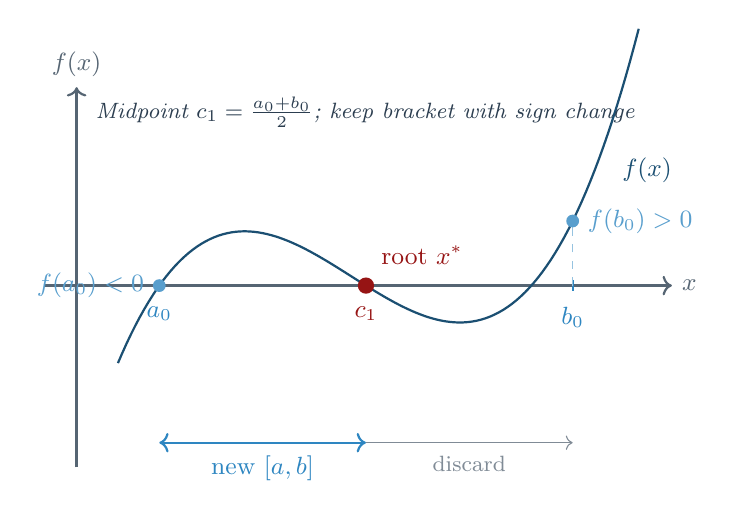
\begin{tikzpicture}[scale=1.05, font=\small]
  % axes
  \draw[->, thick, darktext!80] (-0.4,0) -- (7.2,0) node[right] {$x$};
  \draw[->, thick, darktext!80] (0,-2.2) -- (0,2.4) node[above] {$f(x)$};
  % curve f(x) crossing at x~3.5
  \draw[thick, primary, domain=0.5:6.8, samples=120]
    plot (\x, {0.25*(\x-1)*(\x-3.5)*(\x-5.5)/2});
  \node[primary] at (6.9,1.4) {$f(x)$};
  % bracket a0, b0
  \draw[accent, thick] (1, 0.07) -- (1,-0.07) node[below=2pt] {$a_0$};
  \draw[accent, thick] (6, 0.07) -- (6,-0.07) node[below=2pt] {$b_0$};
  \draw[dashed, accent!50] (1,0) -- (1,{0.25*(1-1)*(1-3.5)*(1-5.5)/2});
  \draw[dashed, accent!50] (6,0) -- (6,{0.25*(6-1)*(6-3.5)*(6-5.5)/2});
  \fill[accent!80] (1,{0.25*(1-1)*(1-3.5)*(1-5.5)/2}) circle (2.2pt) node[left=2pt] {$f(a_0)<0$};
  \fill[accent!80] (6,{0.25*(6-1)*(6-3.5)*(6-5.5)/2}) circle (2.2pt) node[right=2pt] {$f(b_0)>0$};
  % midpoint c1 = 3.5
  \draw[redclr, thick] (3.5,0.07) -- (3.5,-0.07) node[below=2pt] {$c_1$};
  \draw[dashed, redclr!60] (3.5,0) -- (3.5,{0.25*(3.5-1)*(3.5-3.5)*(3.5-5.5)/2});
  \fill[redclr] (3.5,0) circle (2.8pt);
  \node[redclr, above right=2pt] at (3.5,0.07) {root $x^*$};
  % iteration arrows below axis
  \draw[<->, accent, thick] (1,-1.9) -- (3.5,-1.9) node[midway, below=1pt] {new $[a,b]$};
  \draw[->, darktext!60] (3.5,-1.9) -- (6,-1.9);
  \node[darktext!60] at (4.75,-2.15) {\footnotesize discard};
  % label
  \node[darktext, align=center] at (3.5,2.1) {\footnotesize\textit{Midpoint $c_1 = \tfrac{a_0+b_0}{2}$; keep bracket with sign change}};
\end{tikzpicture}
\end{center}

\newpage

\section*{Mathematical Foundation}

\begin{defbox}[Bisection Algorithm]
Given a continuous function $f$ on $[a_0,b_0]$ with $f(a_0)\cdot f(b_0)<0$, at each step $n=0,1,2,\ldots$:
\begin{enumerate}[noitemsep]
  \item Compute the midpoint: $c_n = \dfrac{a_n+b_n}{2}$
  \item If $f(c_n) = 0$: exact root found; stop.
  \item If $f(a_n)\cdot f(c_n) < 0$: root in $[a_n,c_n]$; set $a_{n+1}=a_n,\;b_{n+1}=c_n$.
  \item If $f(c_n)\cdot f(b_n) < 0$: root in $[c_n,b_n]$; set $a_{n+1}=c_n,\;b_{n+1}=b_n$.
  \item Repeat until stopping criterion is met.
\end{enumerate}
The sequence of midpoints $\{c_n\}$ converges to a root $x^*$.
\end{defbox}

\bigskip

\begin{thmbox}[Convergence of Bisection --- Nested Interval Theorem]
Let $f$ be continuous on $[a_0,b_0]$ with $f(a_0)\cdot f(b_0)<0$. The Bisection Method produces nested intervals $[a_n,b_n]$ satisfying:
\begin{enumerate}[noitemsep]
  \item \textbf{Nesting:} $[a_0,b_0]\supset[a_1,b_1]\supset[a_2,b_2]\supset\cdots$
  \item \textbf{Bracketing:} $f(a_n)\cdot f(b_n)<0$ for all $n$.
  \item \textbf{Width:} $b_n-a_n = \dfrac{b_0-a_0}{2^n}$
  \item \textbf{Convergence:} $\{a_n\}$ (non-decreasing, bounded above) and $\{b_n\}$ (non-increasing, bounded below) both converge to the same limit $x^*\in[a_0,b_0]$ with $f(x^*)=0$.
\end{enumerate}
\textbf{Proof of (iv):} By (iii), $b_n-a_n\to 0$. By the Monotone Convergence Theorem, $\{a_n\}\to x^*$ and $\{b_n\}\to x^*$. By (ii) and continuity of $f$: taking limits gives $[f(x^*)]^2\leq 0$, so $f(x^*)=0$.\hfill$\square$
\end{thmbox}

\bigskip

\subsection*{Error Analysis}

After $n$ iterations starting from interval $[a_0, b_0]$, the interval has length:
\[
  b_n - a_n = \frac{b_0 - a_0}{2^n}
\]
The root $x^*$ always lies inside $[a_n, b_n]$, so the \textbf{absolute error bound} is:
\[
  \boxed{|x_n - x^*| \leq \frac{b_0 - a_0}{2^n}}
\]

\begin{thmbox}[Number of Iterations Required]
To achieve an error less than $\varepsilon$, the number of iterations $n$ must satisfy:
\[
  \frac{b_0 - a_0}{2^n} < \varepsilon
  \quad\Longrightarrow\quad
  n > \frac{\ln\!\left(\dfrac{b_0 - a_0}{\varepsilon}\right)}{\ln 2}
  = \log_2\!\left(\frac{b_0 - a_0}{\varepsilon}\right)
\]
\end{thmbox}

\bigskip

\subsection*{Convergence Analysis}

\begin{thmbox}[Linear Convergence of Bisection]
Bisection converges \textbf{linearly} with convergence ratio $\tfrac{1}{2}$:
\[
  |e_{n+1}| \leq \frac{1}{2}|e_n|
  \qquad\text{where}\quad e_n = x_n - x^*
\]
Each iteration reduces the error by exactly half, regardless of the behavior of $f$.
\end{thmbox}

\begin{keybox}
\textbf{Key Insight:} Bisection ignores the actual values $f(a)$ and $f(b)$ — it only uses their \textit{signs}. This makes it very robust (guaranteed convergence) but also inefficient (slow, wastes information about how large or small $f$ is).
\end{keybox}

\bigskip

\subsection*{Stopping Criteria Specific to Bisection}

For Bisection, the interval-width criterion is always preferred (we have a guaranteed bound):
\begin{enumerate}[noitemsep]
  \item \textbf{Primary:} $|b_n-a_n|<2\varepsilon$, ensuring $|c_n-x^*|<\varepsilon$.
  \item \textbf{Secondary:} Also check $|f(c_n)|<\varepsilon_f$ for a function tolerance.
  \item \textbf{Safety:} Always set a maximum iteration count $N_{\max}$ (computable from the formula above).
\end{enumerate}

\begin{keybox}
\textbf{Caution:} The relative change criterion $|c_n-c_{n-1}|/|c_n|$ can be unreliable when $c_n\approx 0$.
\end{keybox}

\subsection*{When Bisection Fails}

\begin{enumerate}[noitemsep]
  \item \textbf{Discontinuous functions:} IVT requires continuity. $f(x)=1/x$ has $f(-1)=-1$ and $f(1)=1$, but $f$ has a pole at 0, not a root.
  \item \textbf{Even-multiplicity roots:} $f(x)=(x-x^*)^2\geq 0$ — no sign change, Bisection cannot locate $x^*$.
  \item \textbf{Multiple roots in bracket:} If there are an odd number of roots in $[a,b]$, Bisection finds one, but not necessarily the desired one.
  \item \textbf{Flat functions:} Round-off in evaluating $\text{sign}(f(c_n))$ may be incorrect if $f(c_n)\approx 0$ at machine precision.
\end{enumerate}

\subsection*{Application: Eigenvalue Computation via Sturm Sequences}

A remarkable application of Bisection is computing eigenvalues of symmetric tridiagonal matrices. The \textbf{Sturm sequence property} allows the number of eigenvalues less than any value $\lambda$ to be computed in $\mathcal{O}(n)$ operations. Combined with Bisection on the parameter $\lambda$, this gives a numerically stable $\mathcal{O}(n\log(1/\varepsilon))$ algorithm — still used in modern linear algebra libraries (LAPACK's \texttt{dstebz}).

\bigskip

\begin{multicols}{2}
\begin{prosbox}
\begin{itemize}[noitemsep]
  \item Guaranteed convergence (IVT)
  \item Simple to implement correctly
  \item No derivative required
  \item A priori error bound (predictable)
  \item Never diverges or gets stuck
  \item Number of iterations known in advance
  \item Works for any continuous $f$
\end{itemize}
\end{prosbox}

\columnbreak

\begin{consbox}
\begin{itemize}[noitemsep]
  \item Slow: linear convergence, factor $=0.5$
  \item Requires initial bracket with sign change
  \item Ignores function magnitude (wastes info)
  \item Cannot find complex roots
  \item Cannot detect even-multiplicity roots
  \item Only finds one root per bracket
  \item Not easily extended to higher dimensions
\end{itemize}
\end{consbox}
\end{multicols}

\newpage

\addcontentsline{toc}{section}{Regula Falsi Method}
% ════════════════════════════════════════════════════════════
%  METHOD 02 — REGULA FALSI
% ════════════════════════════════════════════════════════════

\begin{tcolorbox}[
  enhanced, arc=0pt, boxrule=0pt,
  colback=primary, colframe=primary,
  left=16pt, right=16pt, top=14pt, bottom=10pt,
  borderline south={4pt}{0pt}{accent},
]
  {\color{accent!70}\small\bfseries METHOD 02}\\[4pt]
  {\LARGE\bfseries\color{white} Regula Falsi Method \normalsize\color{lightbg}\quad(False Position)}
\end{tcolorbox}

\vspace{10pt}

\begin{histbox}
The Regula Falsi (Latin for \textit{Rule of False Position}) is one of the \textbf{oldest known root-finding algorithms}, appearing in ancient Egyptian mathematics (circa 1550 BCE, Rhind Papyrus), ancient Babylonian texts, and Indian mathematics (Bakshali manuscript). Medieval Arab mathematicians including Al-Khawarizmi developed it further. It predates calculus by thousands of years and was the dominant algebraic technique until Newton's method emerged in the 17th century. It was formalized in its modern bracket-preserving form during the development of numerical analysis.
\end{histbox}

\bigskip

\begin{center}
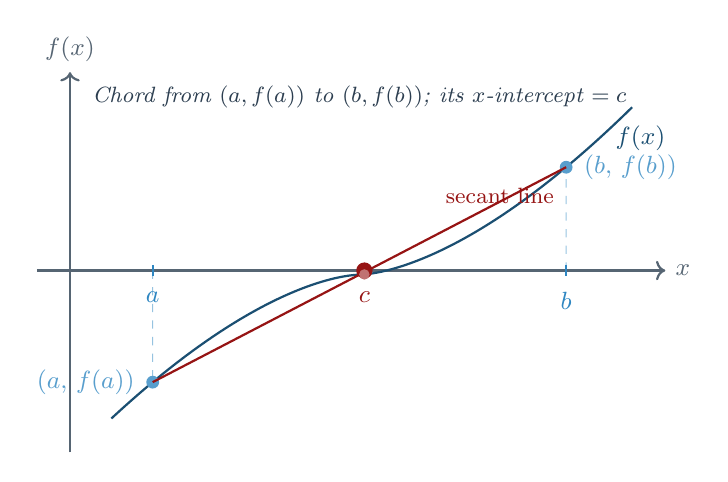
\begin{tikzpicture}[scale=1.05, font=\small]
  % axes
  \draw[->, thick, darktext!80] (-0.4,0) -- (7.2,0) node[right] {$x$};
  \draw[->, thick, darktext!80] (0,-2.2) -- (0,2.4) node[above] {$f(x)$};
  % curve
  \draw[thick, primary, domain=0.5:6.8, samples=120]
    plot (\x, {0.3*(\x-3.5)*abs(\x-3.5)^0.6 - 0.05});
  \node[primary] at (6.9,1.6) {$f(x)$};
  % points a and b
  \coordinate (A) at (1, {0.3*(1-3.5)*abs(1-3.5)^0.6 - 0.05});
  \coordinate (B) at (6, {0.3*(6-3.5)*abs(6-3.5)^0.6 - 0.05});
  \draw[dashed, accent!50] (1,0) -- (A);
  \draw[dashed, accent!50] (6,0) -- (B);
  \fill[accent!80] (A) circle (2.2pt) node[left=3pt] {$(a,\,f(a))$};
  \fill[accent!80] (B) circle (2.2pt) node[right=3pt] {$(b,\,f(b))$};
  \draw[accent, thick] (1,0.07) -- (1,-0.07) node[below=2pt] {$a$};
  \draw[accent, thick] (6,0.07) -- (6,-0.07) node[below=2pt] {$b$};
  % chord (false position line)
  \draw[redclr, thick] (A) -- (B);
  % x-intercept of chord: linear interpolation
  % x_intercept = a - f(a)*(b-a)/(f(b)-f(a))
  % fa = 0.3*(1-3.5)*|1-3.5|^0.6 - 0.05 ≈ -1.97, fb ≈ 1.88
  % c = 1 - (-1.97)*(5)/( 1.88 - (-1.97)) = 1 + 9.85/3.85 ≈ 3.56
  \coordinate (C) at (3.56, 0);
  \draw[redclr, thick] (3.56,0.07) -- (3.56,-0.07) node[below=2pt] {\textcolor{redclr}{$c$}};
  \fill[redclr] (C) circle (2.8pt);
  \draw[dashed, redclr!60] (3.56,0) -- (3.56, {0.3*(3.56-3.5)*abs(3.56-3.5)^0.6 - 0.05});
  \fill[redclr!60] (3.56, {0.3*(3.56-3.5)*abs(3.56-3.5)^0.6 - 0.05}) circle (1.8pt);
  % annotation
  \node[darktext, align=center] at (3.5,2.1)
    {\footnotesize\textit{Chord from $(a,f(a))$ to $(b,f(b))$; its $x$-intercept $= c$}};
  \node[redclr] at (5.2,0.9) {\footnotesize secant line};
\end{tikzpicture}
\end{center}

\newpage

\section*{Mathematical Foundation}

\begin{defbox}[Geometric Interpretation]
Rather than taking the midpoint of $[a,b]$, Regula Falsi draws a \textbf{straight line} (secant line) connecting the points $(a,\,f(a))$ and $(b,\,f(b))$, then uses the $x$-intercept of this line as the next approximation.

\medskip
From the equation of the line through two points:
\[
  \frac{x - a}{b - a} = \frac{0 - f(a)}{f(b) - f(a)}
\]
Solving for $x$ gives the \textbf{false position formula}:
\[
  \boxed{x_n = \frac{a\,f(b) - b\,f(a)}{f(b) - f(a)} = b - f(b)\cdot\frac{b-a}{f(b)-f(a)}}
\]
\end{defbox}

\bigskip

\begin{derivbox}[Formula from Similar Triangles]
Consider the two right triangles formed by the secant line cutting the $x$-axis at $x_n$:
\[
  \frac{x_n - a}{b - x_n} = \frac{|f(a)|}{|f(b)|}
\]
\[
  (x_n - a)|f(b)| = (b - x_n)|f(a)|
\]
\[
  x_n\bigl[|f(b)| + |f(a)|\bigr] = b|f(a)| + a|f(b)|
\]
When $f(a) < 0$ and $f(b) > 0$, accounting for signs gives the standard formula.
\end{derivbox}

\bigskip

\subsection*{The Algorithm}

\begin{defbox}[Regula Falsi Algorithm]
Given $[a_0,b_0]$ with $f(a_0)\cdot f(b_0)<0$:
\begin{enumerate}[noitemsep]
  \item Compute: $c_n = \dfrac{a_n f(b_n)-b_n f(a_n)}{f(b_n)-f(a_n)}$
  \item If $f(c_n)=0$: root found; stop.
  \item If $f(a_n)\cdot f(c_n)<0$: set $b_{n+1}=c_n,\;a_{n+1}=a_n$.
  \item Else: set $a_{n+1}=c_n,\;b_{n+1}=b_n$.
  \item Repeat until $|f(c_n)|<\varepsilon$ or $|b_n-a_n|<\delta$.
\end{enumerate}
\end{defbox}

\subsection*{Convergence Analysis and Stagnation}

Regula Falsi always converges (bracket maintained). However, it suffers from a well-known pathology:

\begin{thmbox}[One-Sided Convergence --- Stagnation Theorem]
If $f$ is convex ($f''>0$) on $[a,b]$ with root $x^*\in(a,b)$ and $f(a)<0<f(b)$, then $b$ is retained at every step: $b_n=b_0$ for all $n$. Only the left endpoint $a_n\to x^*$. Convergence is linear with rate:
\[
  \lim_{n\to\infty}\frac{|e_{n+1}|}{|e_n|} = 1 - \frac{f'(x^*)}{f'(x^*)+K} < 1
\]
where $K$ is related to the curvature of $f$ at $x^*$. This ratio can be very close to 1, making convergence extremely slow for highly curved functions.

\medskip
\textbf{Intuition:} Since $f$ is convex, the chord lies above the curve, so its $x$-intercept is always to the right of $x^*$ — the right bracket never tightens.
\end{thmbox}

\subsection*{Improved Variants}

\begin{defbox}[Illinois Algorithm --- Dowell \& Jarratt, 1971]
If the same endpoint (say $b$) is retained for two consecutive iterations, replace its function value with half:
\[
  \tilde{f}(b) \leftarrow \tfrac{f(b)}{2}
\]
This artificially reduces the weight given to the stagnant endpoint, forcing $c$ to move further into the bracket. Achieves \textbf{superlinear convergence} (order $\approx 1.44$) while maintaining the bracket guarantee.
\end{defbox}

\begin{defbox}[Pegasus Method --- Dowell \& Jarratt, 1972]
When the same endpoint $b$ is retained, replace:
\[
  \tilde{f}(b) \leftarrow f(b)\cdot\frac{f(b_\text{old})}{f(b_\text{old})+f(c)}
\]
A more sophisticated weighting than Illinois, achieving convergence order $\approx 1.64$ — very close to the Secant Method's golden-ratio order.
\end{defbox}

\begin{defbox}[Anderson-Björck Method --- 1973]
Adapts the weight dynamically:
\[
  \tilde{f}(b) \leftarrow f(b)\cdot\max\!\left(\tfrac{1}{2},\;1-\tfrac{f(c)}{f(b)}\right)
\]
Also achieves order $\approx 1.64$ and adapts based on current function values.
\end{defbox}

\begin{center}{\footnotesize\setlength{\tabcolsep}{4pt}
\begin{tabular}{p{3.5cm} C{2.2cm} C{2.4cm} C{2.4cm} C{2.8cm}}
\toprule
\rowcolor{primary}
\hcell{Method} & \hcell{Conv.\ Order} & \hcell{Bracket?} & \hcell{Extra Cost} & \hcell{Note} \\
\midrule
\rowcolor{amberbg}
Regula Falsi (plain) & 1 (stagnates) & Yes & None & May be very slow \\
Illinois & $\approx 1.44$ & Yes & One test/step & Simple fix \\
\rowcolor{amberbg}
Pegasus & $\approx 1.64$ & Yes & One multiply & Best of variants \\
Anderson-Björck & $\approx 1.64$ & Yes & One comparison & Adaptive \\
\rowcolor{amberbg}
Brent's Method & up to $\approx 1.618$ & Yes & Moderate & Production gold standard \\
\bottomrule
\end{tabular}
}\end{center}

\subsection*{Engineering Applications}

Regula Falsi and its variants are widely used because they guarantee convergence without requiring derivatives:
\begin{itemize}[noitemsep]
  \item \textbf{Pipe-flow:} Colebrook--White equation for friction factor (transcendental in $f$).
  \item \textbf{Thermodynamics:} Van der Waals equation of state for $V$.
  \item \textbf{Circuit analysis:} Diode equations with exponential nonlinearities.
  \item \textbf{Structural mechanics:} Buckling load equations.
\end{itemize}

\bigskip

\begin{multicols}{2}
\begin{prosbox}
\begin{itemize}[noitemsep]
  \item Bracket always maintained (safe)
  \item Uses slope information (smarter than bisection)
  \item Faster than bisection in most cases
  \item Guaranteed convergence
  \item No derivative required
\end{itemize}
\end{prosbox}

\columnbreak

\begin{consbox}
\begin{itemize}[noitemsep]
  \item One endpoint may stagnate (slow)
  \item Still only linear convergence
  \item Slower than Newton-Raphson / Secant
  \item Requires initial bracket
  \item Poor for nearly flat $f$ near root
\end{itemize}
\end{consbox}
\end{multicols}

\newpage

\addcontentsline{toc}{section}{Newton-Raphson Method}
% ════════════════════════════════════════════════════════════
%  METHOD 03 — NEWTON-RAPHSON
% ════════════════════════════════════════════════════════════

\begin{tcolorbox}[
  enhanced, arc=0pt, boxrule=0pt,
  colback=primary, colframe=primary,
  left=16pt, right=16pt, top=14pt, bottom=10pt,
  borderline south={4pt}{0pt}{accent},
]
  {\color{accent!70}\small\bfseries METHOD 03}\\[4pt]
  {\LARGE\bfseries\color{white} Newton-Raphson Method}
\end{tcolorbox}

\vspace{10pt}

\begin{histbox}
\textbf{Isaac Newton} (1669, \textit{De analysi}) introduced a version of this method for polynomials. \textbf{Joseph Raphson} (1690) independently published a simplified, more general algebraic form. The modern calculus-based form using $f'(x)$ was developed by \textbf{Thomas Simpson} (1740). The method is now considered the cornerstone of computational root finding and is the basis of numerical solvers in MATLAB, Python's \texttt{scipy.optimize}, and virtually every scientific computing library.
\end{histbox}

\bigskip

\begin{center}
\begin{tikzpicture}[scale=1.1, font=\small]
  % axes
  \draw[->, thick, darktext!80] (-0.4,0) -- (7,0) node[right] {$x$};
  \draw[->, thick, darktext!80] (0,-1.2) -- (0,3.2) node[above] {$f(x)$};
  % curve f(x) = (x-2)^2 - 0.5, root near x=2.71
  \draw[thick, primary, domain=0.5:6.5, samples=120]
    plot (\x, {0.4*(\x-2)*(\x-2) - 0.6});
  \node[primary] at (6.6,1.8) {$f(x)$};
  % x0 = 5
  \def\xz{5}
  \def\fxz{0.4*(5-2)*(5-2) - 0.6}  % = 3.0
  \def\dfxz{0.8*(5-2)}              % = 2.4
  % tangent at x0: y - fxz = dfxz*(x - xz)  =>  y = dfxz*x - dfxz*xz + fxz
  % x-intercept: 0 = dfxz*x - dfxz*xz + fxz => x = xz - fxz/dfxz = 5 - 3/2.4 = 3.75
  \def\xone{3.75}
  \def\fxone{0.4*(3.75-2)*(3.75-2) - 0.6}  % = 0.4*3.0625 - 0.6 = 0.625
  \def\dfxone{0.8*(3.75-2)}                  % = 1.4
  % x2 = x1 - f(x1)/f'(x1) = 3.75 - 0.625/1.4 = 3.304
  \def\xtwo{3.30}
  % draw tangent at x0
  \draw[redclr, thick] (2.5, {\dfxz*2.5 - \dfxz*\xz + \fxz}) -- (5.5, {\dfxz*5.5 - \dfxz*\xz + \fxz});
  % vertical dashed lines
  \draw[dashed, accent!50] (\xz,0) -- (\xz,{\fxz});
  \draw[dashed, accent!50] (\xone,0) -- (\xone,{\fxone});
  \draw[dashed, accent!50] (\xtwo,0) -- (\xtwo,{0.4*(\xtwo-2)*(\xtwo-2)-0.6});
  % points on curve
  \fill[primary] (\xz,{\fxz}) circle (2.5pt);
  \fill[primary] (\xone,{\fxone}) circle (2.5pt);
  % x labels
  \draw[accent, thick] (\xz,0.07) -- (\xz,-0.07) node[below=2pt] {$x_0$};
  \draw[accent, thick] (\xone,0.07) -- (\xone,-0.07) node[below=2pt] {$x_1$};
  \draw[redclr, thick] (\xtwo,0.07) -- (\xtwo,-0.07) node[below=2pt] {$x_2$};
  % tangent at x1
  \draw[redclr!70, thick, dashed]
    (2.8, {\dfxone*2.8 - \dfxone*\xone + \fxone}) --
    (4.2, {\dfxone*4.2 - \dfxone*\xone + \fxone});
  % arrows showing iteration direction
  \draw[->, thick, accent!70] (\xz+0.05,-0.5) -- (\xone+0.05,-0.5);
  \draw[->, thick, accent!40] (\xone+0.05,-0.7) -- (\xtwo+0.05,-0.7);
  % root marker
  \fill[greenclr] (2.72,0) circle (2.5pt) node[above right=1pt] {\footnotesize\color{greenclr}$x^*$};
  % label
  \node[darktext, align=center] at (3.5,2.8)
    {\footnotesize\textit{Tangent at $x_n$ crosses $x$-axis $\Rightarrow x_{n+1} = x_n - f(x_n)/f'(x_n)$}};
\end{tikzpicture}
\end{center}

\newpage

\section*{Derivation}

\begin{derivbox}[From Taylor Series Expansion]
Expand $f(x)$ in a Taylor series about the current estimate $x_n$:
\[
  f(x) = f(x_n) + (x - x_n)f'(x_n) + \frac{(x-x_n)^2}{2!}f''(x_n) + \cdots
\]
Truncate after the \textbf{linear term} (linear approximation):
\[
  f(x) \approx f(x_n) + (x - x_n)f'(x_n)
\]
Set $f(x) = 0$ and solve for $x$:
\[
  0 = f(x_n) + (x_{n+1} - x_n)f'(x_n)
\]
\[
  \boxed{x_{n+1} = x_n - \frac{f(x_n)}{f'(x_n)}}
\]
\end{derivbox}

\bigskip

\begin{defbox}[Geometric Interpretation]
At each step, draw the \textbf{tangent line} to the curve $y = f(x)$ at the point $(x_n,\,f(x_n))$. The tangent line has equation:
\[
  y - f(x_n) = f'(x_n)(x - x_n)
\]
Setting $y = 0$ gives $x_{n+1}$. The method thus ``slides down the slope'' toward the root. This is why the method fails when $f'(x_n) = 0$ (horizontal tangent).
\end{defbox}

\bigskip

\subsection*{Convergence Analysis}

\begin{thmbox}[Quadratic Convergence]
Assume $f$ has a \textbf{simple root} $x^*$ (i.e., $f(x^*) = 0$ and $f'(x^*) \neq 0$), and that $f''$ is continuous near $x^*$. Then Newton-Raphson converges \textbf{quadratically}:
\[
  |e_{n+1}| \approx \frac{|f''(x^*)|}{2|f'(x^*)|}|e_n|^2
  \qquad\text{where}\quad e_n = x_n - x^*
\]
The constant $C = \dfrac{|f''(x^*)|}{2|f'(x^*)|}$ is called the \textbf{asymptotic error constant}.

\medskip
\textbf{Practical consequence:} If $|e_n| = 10^{-3}$, then $|e_{n+1}| \approx C \times 10^{-6}$ --- the number of correct decimal digits approximately \textit{doubles} at each step.
\end{thmbox}

\bigskip

\subsection*{Convergence Theorems}

\begin{thmbox}[Local Convergence Theorem]
Suppose $f:[a,b]\to\mathbb{R}$ is twice continuously differentiable, $f(x^*)=0$, and $f'(x^*)\neq 0$. Then there exists $\delta>0$ such that for any $x_0$ with $|x_0-x^*|<\delta$, Newton-Raphson converges quadratically to $x^*$.

\medskip
\textbf{Proof sketch:} Since $f'$ is continuous and $f'(x^*)\neq 0$, there exists $\delta>0$ with $|f'(x)|\geq m>0$ on $[x^*-\delta,x^*+\delta]$ and $|f''(x)|\leq M$. Then:
\[
  |e_{n+1}| = \frac{|f''(\xi_n)|}{2|f'(x_n)|}|e_n|^2 \leq \frac{M}{2m}|e_n|^2
\]
If $|e_0|<2m/M$, then $|e_n|<\delta$ for all $n$ by induction.\hfill$\square$
\end{thmbox}

\begin{thmbox}[Fourier--Kantorovich Sufficient Condition]
If $f,f',f''$ are continuous on $[a,b]$, $f(a)\cdot f(b)<0$, and for all $x\in[a,b]$:
\[
  \frac{f(x)\,f''(x)}{[f'(x)]^2} < 1
\]
Then Newton-Raphson converges monotonically to $x^*$, provided $x_0$ is chosen as the endpoint satisfying $f(x_0)\cdot f''(x_0)>0$ (i.e.\ $f$ and $f''$ have the same sign).
\end{thmbox}

\bigskip

\subsection*{Failure Cases}

\begin{keybox}
\textbf{When Newton-Raphson Fails or Diverges:}
\begin{enumerate}[noitemsep]
  \item \textbf{$f'(x_n) = 0$}: Division by zero — method is undefined. Occurs at stationary points.
  \item \textbf{Inflection point near root}: Tangent lines ``shoot off'' to infinity.
  \item \textbf{Cycling}: For some functions and starting points, the iteration oscillates between two values.
  \item \textbf{Divergence}: If $x_0$ is far from $x^*$ or $f$ is highly nonlinear, the method may diverge.
  \item \textbf{Wrong root}: May converge to a different root than intended.
\end{enumerate}
\end{keybox}

\bigskip

\subsection*{Newton-Raphson for Systems of Equations}

Newton-Raphson generalises to systems $\mathbf{F}(\mathbf{x})=\mathbf{0}$ where $\mathbf{F}:\mathbb{R}^n\to\mathbb{R}^n$:
\[
  \mathbf{x}_{n+1} = \mathbf{x}_n - J(\mathbf{x}_n)^{-1}\mathbf{F}(\mathbf{x}_n)
\]
where $J(\mathbf{x}_n)$ is the \textbf{Jacobian matrix} with entries $J_{ij}=\partial F_i/\partial x_j$. In practice, one solves the linear system $J(\mathbf{x}_n)\,\boldsymbol{\delta}=-\mathbf{F}(\mathbf{x}_n)$ and sets $\mathbf{x}_{n+1}=\mathbf{x}_n+\boldsymbol{\delta}$.

\subsection*{Halley's Method: Cubic Convergence}

\begin{defbox}[Halley's Method --- Edmond Halley, 1694]
Uses a second-order Taylor approximation (osculating parabola) instead of a tangent line:
\[
  x_{n+1} = x_n - \frac{2f(x_n)f'(x_n)}{2[f'(x_n)]^2 - f(x_n)f''(x_n)}
\]
Convergence order is $p=3$: $|e_{n+1}|\approx \dfrac{|f'''(x^*)|}{3|f'(x^*)|}|e_n|^3$. Correct digits triple each step. However, $f''$ is also required, increasing computational cost.
\end{defbox}

\subsection*{Basin of Attraction}

For complex-valued functions, the set of starting points converging to a particular root under Newton iteration forms the \textbf{basin of attraction} for that root. For polynomials, these basins are \textbf{fractals} — the famous \textit{Newton fractals} — with boundaries intimately related to Julia sets in complex dynamics. This demonstrates that even a simple algorithm can exhibit extraordinary sensitivity to initial conditions.

\subsection*{Modified Newton-Raphson for Multiple Roots}

When $x^*$ is a root of \textbf{multiplicity} $m$ (i.e., $f(x^*) = f'(x^*) = \cdots = f^{(m-1)}(x^*) = 0$), standard Newton-Raphson degenerates to \textit{linear} convergence. The fix:

\begin{defbox}[Modified Formula for Multiple Roots]
\[
  x_{n+1} = x_n - m\cdot\frac{f(x_n)}{f'(x_n)}
\]
or equivalently, define $u(x) = \dfrac{f(x)}{f'(x)}$ and apply Newton to $u(x) = 0$:
\[
  x_{n+1} = x_n - \frac{u(x_n)}{u'(x_n)} = x_n - \frac{f(x_n)f'(x_n)}{[f'(x_n)]^2 - f(x_n)f''(x_n)}
\]
This \textbf{restores quadratic convergence} for multiple roots.
\end{defbox}

\bigskip

\begin{multicols}{2}
\begin{prosbox}
\begin{itemize}[noitemsep]
  \item Quadratic convergence (very fast)
  \item Correct digits double each step
  \item Foundation of many advanced solvers
  \item Easily extended to systems of equations
  \item Works in complex plane
\end{itemize}
\end{prosbox}

\columnbreak

\begin{consbox}
\begin{itemize}[noitemsep]
  \item Requires $f'(x)$ (may be hard to compute)
  \item Only local convergence (sensitive to $x_0$)
  \item Fails if $f'(x_n) = 0$
  \item May converge to wrong root
  \item Slow for multiple roots (unless modified)
\end{itemize}
\end{consbox}
\end{multicols}

\newpage

\addcontentsline{toc}{section}{Secant Method}
% ════════════════════════════════════════════════════════════
%  METHOD 04 — SECANT
% ════════════════════════════════════════════════════════════

\begin{tcolorbox}[
  enhanced, arc=0pt, boxrule=0pt,
  colback=primary, colframe=primary,
  left=16pt, right=16pt, top=14pt, bottom=10pt,
  borderline south={4pt}{0pt}{accent},
]
  {\color{accent!70}\small\bfseries METHOD 04}\\[4pt]
  {\LARGE\bfseries\color{white} Secant Method}
\end{tcolorbox}

\vspace{10pt}

\begin{histbox}
The Secant Method is closely related to Regula Falsi and has roots going back to ancient times, but its modern derivative-free formulation is attributed to \textbf{18th-century numerical analysts}. The method gained prominence as a practical alternative to Newton-Raphson when derivatives are difficult to compute symbolically. It is particularly important in \textbf{quasi-Newton optimization methods} (BFGS, SR1) and in the solution of nonlinear systems. The remarkable result that its convergence order is the \textit{golden ratio} $\varphi = \frac{1+\sqrt{5}}{2}$ was established through careful error analysis.
\end{histbox}

\bigskip

\begin{center}
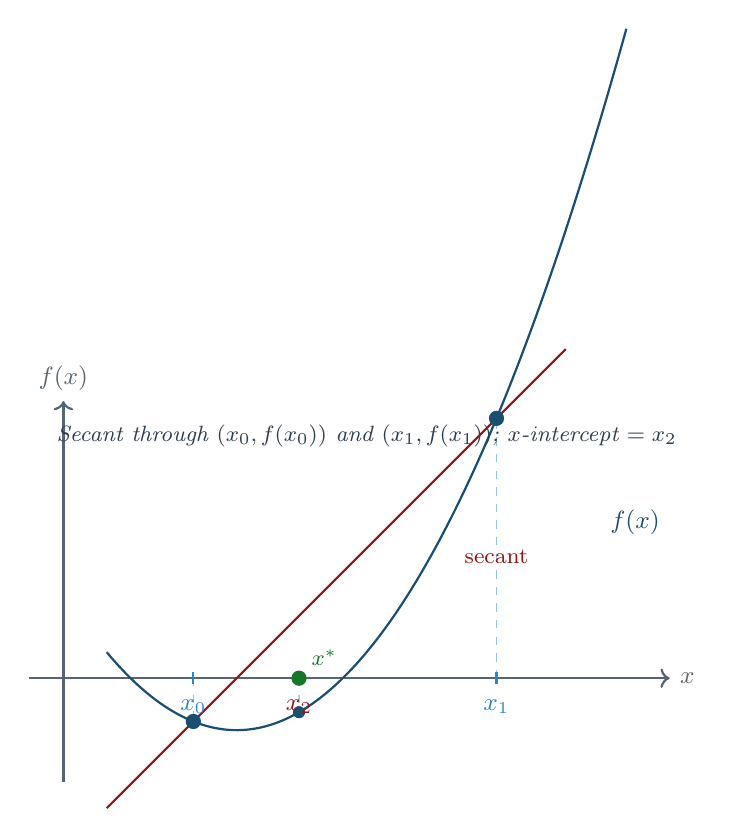
\begin{tikzpicture}[scale=1.1, font=\small]
  % axes
  \draw[->, thick, darktext!80] (-0.4,0) -- (7,0) node[right] {$x$};
  \draw[->, thick, darktext!80] (0,-1.2) -- (0,3.2) node[above] {$f(x)$};
  % curve
  \draw[thick, primary, domain=0.5:6.5, samples=120]
    plot (\x, {0.4*(\x-2)*(\x-2) - 0.6});
  \node[primary] at (6.6,1.8) {$f(x)$};
  % x0=1.2, x1=5
  \def\xz{1.5}   \def\fxz{0.4*(1.5-2)*(1.5-2)-0.6}    % ~-0.5
  \def\xo{5.0}   \def\fxo{0.4*(5-2)*(5-2)-0.6}         % ~3.0
  % secant line 1 through (x0,f(x0)) and (x1,f(x1))
  % slope = (fxo - fxz)/(xo - xz) = (3.0 - (-0.5))/(3.5) = 1.0
  % x-intercept: x2 = x1 - fxo*(xo-xz)/(fxo-fxz) = 5 - 3.0*3.5/3.5 = 5-3 = 2.0?
  % actually x2 = xo - fxo*(xo-xz)/(fxo-fxz)
  \def\xt{2.72}   \def\fxt{0.4*(2.72-2)*(2.72-2)-0.6}  % ~-0.39
  % draw secant line 1
  \draw[redclr, thick] (0.5, {1.0*0.5 - 1.0*\xo + \fxo}) -- (5.8, {1.0*5.8 - 1.0*\xo + \fxo});
  % vertical dashed
  \draw[dashed, accent!50] (\xz,0) -- (\xz,{\fxz});
  \draw[dashed, accent!50] (\xo,0) -- (\xo,{\fxo});
  \draw[dashed, accent!40] (\xt,0) -- (\xt,{\fxt});
  % points on curve
  \fill[primary] (\xz,{\fxz}) circle (2.5pt);
  \fill[primary] (\xo,{\fxo}) circle (2.5pt);
  \fill[primary] (\xt,{\fxt}) circle (2pt);
  % x labels
  \draw[accent, thick] (\xz,0.07) -- (\xz,-0.07) node[below=2pt] {$x_0$};
  \draw[accent, thick] (\xo,0.07) -- (\xo,-0.07) node[below=2pt] {$x_1$};
  \draw[redclr, thick] (\xt,0.07) -- (\xt,-0.07) node[below=2pt] {$x_2$};
  % root
  \fill[greenclr] (2.72,0) circle (2.5pt) node[above right=1pt] {\footnotesize\color{greenclr}$x^*$};
  % label
  \node[darktext, align=center] at (3.5,2.8)
    {\footnotesize\textit{Secant through $(x_0,f(x_0))$ and $(x_1,f(x_1))$; $x$-intercept $= x_2$}};
  \node[redclr] at (5.0,1.4) {\footnotesize secant};
\end{tikzpicture}
\end{center}

\newpage

\section*{Derivation}

\begin{derivbox}[Finite Difference Approximation of Derivative]
Newton-Raphson requires $f'(x_n)$. In the Secant Method, we \textbf{approximate} the derivative using a finite difference between the two most recent iterates:
\[
  f'(x_n) \approx \frac{f(x_n) - f(x_{n-1})}{x_n - x_{n-1}}
\]
Substituting into the Newton-Raphson formula:
\[
  x_{n+1} = x_n - \frac{f(x_n)}{\dfrac{f(x_n) - f(x_{n-1})}{x_n - x_{n-1}}}
\]
\[
  \boxed{x_{n+1} = x_n - f(x_n)\cdot\frac{x_n - x_{n-1}}{f(x_n) - f(x_{n-1})}}
\]
Geometrically, this is the $x$-intercept of the \textbf{secant line} through $(x_{n-1},\,f(x_{n-1}))$ and $(x_n,\,f(x_n))$.
\end{derivbox}

\bigskip

\subsection*{Secant vs.\ Regula Falsi}

\begin{center}
{\small
\begin{tabular}{p{4.5cm} p{4.5cm} p{4.5cm}}
\toprule
\rowcolor{primary}
\hcell{Feature} & \hcell{Regula Falsi} & \hcell{Secant Method} \\
\midrule
\rowcolor{amberbg}
Bracket required & Yes & No \\
Points used & $a$ and $b$ (bracket ends) & $x_{n-1}$ and $x_n$ (last two) \\
\rowcolor{amberbg}
Convergence & Linear (may stagnate) & Superlinear \\
Sign change enforced & Yes & No \\
\rowcolor{amberbg}
Guaranteed convergence & Yes & No \\
\bottomrule
\end{tabular}
}
\end{center}

\bigskip

\subsection*{Convergence Analysis}

\begin{thmbox}[Superlinear Convergence --- Golden Ratio Order]
For a simple root $x^*$ with $f'(x^*)\neq 0$, the Secant Method converges with order $p=\varphi=(1+\sqrt{5})/2\approx 1.618$.
\end{thmbox}

\begin{derivbox}[Proof: Error Recurrence and the Fibonacci Connection]
Let $e_n=x_n-x^*$. Using the divided difference $f[x_{n-1},x_n]=(f(x_n)-f(x_{n-1}))/(x_n-x_{n-1})$ and expanding around $x^*$:
\[
  f(x_n)\approx f'(x^*)e_n + \tfrac{1}{2}f''(x^*)e_n^2, \qquad f[x_{n-1},x_n]\approx f'(x^*) + \tfrac{f''(x^*)}{2}(e_n+e_{n-1})
\]
After simplification, the error satisfies:
\[
  e_{n+1} \approx -\frac{f''(x^*)}{2f'(x^*)}\,e_n\,e_{n-1} = -C\,e_n\,e_{n-1}
\]
Assuming $|e_n|\approx A\lambda^{p^n}$, comparing powers gives $p^{n+1}=p^n+p^{n-1}$, i.e.\ $p^2=p+1$. This is exactly the \textbf{Fibonacci recurrence characteristic equation}, whose positive root is:
\[
  p = \frac{1+\sqrt{5}}{2} \approx 1.618 \qquad\text{(the Golden Ratio }\varphi\text{)}
\]
\textbf{Deep connection:} The Secant error satisfies the same recurrence as Fibonacci numbers. This is why the convergence order equals $\varphi$.\hfill$\square$
\end{derivbox}

\begin{keybox}
\textbf{Numerical Instability Warning:} When $x_n\approx x_{n-1}$ (iterates are close), computing $f(x_n)-f(x_{n-1})$ causes \textbf{catastrophic cancellation}. If both values agree in the first 12 of 15 digits, the difference has only 3 correct digits — the Secant step becomes wildly inaccurate. \textbf{Remedy:} switch to Bisection when $|x_n-x_{n-1}|$ becomes very small. This is exactly what Brent's Method does.
\end{keybox}

\bigskip

\subsection*{Computational Efficiency}

\begin{keybox}
\textbf{Function Evaluation Comparison:}

Newton-Raphson needs $2$ evaluations per step ($f$ and $f'$), achieving quadratic convergence (order 2). The Secant Method needs only $1$ evaluation per step (reusing $f(x_{n-1})$), achieving order 1.618.

\medskip
In terms of evaluations per order gained, Secant is \textbf{more efficient} than Newton-Raphson:
\[
  \text{Newton: } p = 2 \text{ per 2 evals} \quad\leftrightarrow\quad
  \text{Secant: } p \approx 1.618 \text{ per 1 eval}
\]
To get 10 digits with Newton: $\approx 7$ evaluations. To get 10 digits with Secant: $\approx 9$ evaluations. The difference is small, but Secant avoids symbolic differentiation entirely.
\end{keybox}

\bigskip

\subsection*{Extensions}

\begin{defbox}[Muller's Method --- 1956]
While Secant fits a line through \textit{two} points, Muller's Method fits a \textbf{quadratic} through three consecutive iterates $(x_{n-2},f(x_{n-2}))$, $(x_{n-1},f(x_{n-1}))$, $(x_n,f(x_n))$ and takes the nearest root of this quadratic as $x_{n+1}$. Convergence order $p\approx 1.839$ (root of $p^3=p^2+p+1$). Can find \textbf{complex roots} starting from real initial values.
\end{defbox}

\begin{defbox}[Inverse Quadratic Interpolation (IQI)]
Treats $x$ as a function of $f$ and fits a quadratic through $(f(x_{n-2}),x_{n-2})$, $(f(x_{n-1}),x_{n-1})$, $(f(x_n),x_n)$. Evaluating at $f=0$ gives the next iterate. Order $\approx 1.839$, numerically stable (no complex arithmetic). Used as the primary step in Brent's Method.
\end{defbox}

\begin{thmbox}[Brent's Method --- The Practical Gold Standard]
\textbf{Richard Brent, 1973.} A hybrid algorithm combining:
\begin{enumerate}[noitemsep]
  \item \textbf{Inverse Quadratic Interpolation} (fast, order $\approx 1.839$) — used when it makes progress.
  \item \textbf{Secant Method} (fast, order 1.618) — used as fallback.
  \item \textbf{Bisection} (slow but guaranteed) — used when faster methods fail.
\end{enumerate}
Maintains a bracket (guaranteed convergence) while achieving superlinear speed in smooth regions. Implemented as \texttt{scipy.optimize.brentq}, MATLAB's \texttt{fzero}, and in GNU Scientific Library.
\end{thmbox}

\begin{multicols}{2}
\begin{prosbox}
\begin{itemize}[noitemsep]
  \item No derivative required
  \item Superlinear convergence ($\approx 1.618$)
  \item Only 1 function evaluation per step
  \item Higher efficiency index than Newton
  \item Simple formula, easy to implement
  \item Muller extension finds complex roots
\end{itemize}
\end{prosbox}

\columnbreak

\begin{consbox}
\begin{itemize}[noitemsep]
  \item No bracket maintained (may diverge)
  \item Needs two starting values $x_0,x_1$
  \item Catastrophic cancellation near convergence
  \item May converge to wrong root
  \item Slower than Newton per iteration
  \item Fails if $f(x_n)=f(x_{n-1})$
\end{itemize}
\end{consbox}
\end{multicols}

\newpage

\addcontentsline{toc}{section}{Fixed Point Iteration}
% ════════════════════════════════════════════════════════════
%  METHOD 05 — FIXED POINT ITERATION
% ════════════════════════════════════════════════════════════

\begin{tcolorbox}[
  enhanced, arc=0pt, boxrule=0pt,
  colback=primary, colframe=primary,
  left=16pt, right=16pt, top=14pt, bottom=10pt,
  borderline south={4pt}{0pt}{accent},
]
  {\color{accent!70}\small\bfseries METHOD 05}\\[4pt]
  {\LARGE\bfseries\color{white} Fixed Point Iteration}
\end{tcolorbox}

\vspace{10pt}

\begin{histbox}
Fixed point theory is a cornerstone of modern mathematics. The \textbf{Banach Fixed Point Theorem} (Stefan Banach, 1922) provided the rigorous foundation for the convergence of iterative methods in complete metric spaces. L.E.J. Brouwer's topological fixed point theorem (1911) established existence in higher dimensions. In numerical analysis, fixed point iteration underpins many algorithms — including Newton-Raphson (as a special case), the Gauss-Seidel method for linear systems, and iterative solvers in computational physics. The concept of a \textit{contraction mapping} is fundamental across pure and applied mathematics.
\end{histbox}

\bigskip

\begin{center}
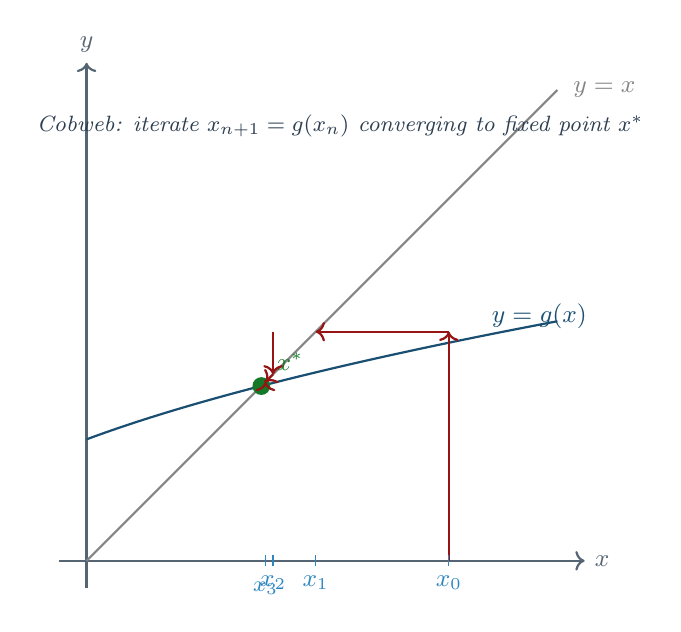
\begin{tikzpicture}[scale=1.15, font=\small]
  % axes
  \draw[->, thick, darktext!80] (-0.3,0) -- (5.5,0) node[right] {$x$};
  \draw[->, thick, darktext!80] (0,-0.3) -- (0,5.5) node[above] {$y$};
  % y = x line
  \draw[thick, grayclr!70, domain=0:5.2] plot(\x,\x) node[right=2pt] {$y=x$};
  % g(x) = sqrt(x+1.5) -- fixed point near x=1.91
  \draw[thick, primary, domain=0:5.2, samples=100]
    plot (\x, {sqrt(\x + 1.8)});
  \node[primary] at (5.0,2.7) {$y=g(x)$};
  % fixed point x* ≈ 1.91 (solving x=sqrt(x+1.8) => x^2=x+1.8 => x=(1+sqrt(8.2))/2 ≈ 1.93)
  \fill[greenclr] (1.93,1.93) circle (2.8pt) node[above right=2pt] {\color{greenclr}$x^*$};
  % cobweb: start x0=4
  \def\xa{4.0}   \def\ga{2.530}   % g(4)=sqrt(5.8)
  \def\xb{2.530} \def\gb{2.059}   % g(2.530)=sqrt(4.33)
  \def\xc{2.059} \def\gc{1.976}   % g(2.059)=sqrt(3.859)
  \def\xd{1.976} \def\gd{1.948}
  % step 1: from (x0,0) up to (x0,g(x0))
  \draw[redclr, thick, ->] (\xa,0) -- (\xa,\ga);
  % step 2: across to y=x: (x0,g(x0)) -> (g(x0),g(x0))
  \draw[redclr, thick, ->] (\xa,\ga) -- (\ga,\ga);
  % step 3: up to g(x1)
  \draw[redclr, thick, ->] (\gb,\ga) -- (\gb,\gb);
  % step 4: across
  \draw[redclr, thick, ->] (\gb,\gb) -- (\gc,\gc);
  % step 5
  \draw[redclr, thick, ->] (\gc,\gc) -- (\gc,\gc);
  % x labels
  \draw[accent] (\xa,0.06) -- (\xa,-0.06) node[below] {$x_0$};
  \draw[accent] (\ga,0.06) -- (\ga,-0.06) node[below] {$x_1$};
  \draw[accent] (\gb,0.06) -- (\gb,-0.06) node[below] {$x_2$};
  \draw[accent] (\gc,0.06) -- (\gc,-0.06) node[below=2pt] {\footnotesize$x_3$};
  % annotation
  \node[darktext, align=center] at (2.8,4.8)
    {\footnotesize\textit{Cobweb: iterate $x_{n+1}=g(x_n)$ converging to fixed point $x^*$}};
\end{tikzpicture}
\end{center}

\newpage

\section*{Mathematical Foundation}

\begin{defbox}[Fixed Point]
A point $x^*$ is a \textbf{fixed point} of a function $g$ if:
\[
  g(x^*) = x^*
\]
To find a root of $f(x) = 0$, we rewrite the equation as $x = g(x)$ for some function $g$. Any fixed point of $g$ is then a root of $f$.

\medskip
\textbf{Examples of rearrangements} for $f(x) = x^3 - 2x - 5 = 0$:
\[
  g_1(x) = \sqrt[3]{2x+5} \quad\text{(converges)}\qquad
  g_2(x) = \frac{x^3 - 5}{2} \quad\text{(diverges)}
\]
The key is choosing $g$ so that $|g'(x^*)| < 1$.
\end{defbox}

\bigskip

\begin{thmbox}[Banach Fixed Point Theorem (Contraction Mapping Theorem)]
Let $g$ be a \textbf{contraction mapping} on a closed interval $[a,b]$, meaning:
\begin{enumerate}[noitemsep]
  \item $g(x) \in [a,b]$ for all $x \in [a,b]$ \hfill(self-mapping)
  \item $|g(x) - g(y)| \leq L|x - y|$ for all $x,y \in [a,b]$, where $0 \leq L < 1$ \hfill(Lipschitz condition)
\end{enumerate}
Then:
\begin{itemize}[noitemsep]
  \item $g$ has a \textbf{unique fixed point} $x^*$ in $[a,b]$.
  \item The iteration $x_{n+1} = g(x_n)$ \textbf{converges} to $x^*$ for any $x_0 \in [a,b]$.
  \item Error bound: $|x_n - x^*| \leq \dfrac{L^n}{1-L}|x_1 - x_0|$
\end{itemize}
\end{thmbox}

\bigskip

\begin{derivbox}[Convergence Condition via Derivative]
By the Mean Value Theorem, if $g$ is differentiable on $[a,b]$:
\[
  g(x_n) - g(x^*) = g'(\xi_n)(x_n - x^*)
  \quad\text{for some } \xi_n \text{ between } x_n \text{ and } x^*
\]
Therefore:
\[
  e_{n+1} = x_{n+1} - x^* = g(x_n) - g(x^*) = g'(\xi_n)\,e_n
\]
As $x_n \to x^*$, we get $\xi_n \to x^*$, so asymptotically:
\[
  |e_{n+1}| \approx |g'(x^*)|\,|e_n|
\]
The convergence rate is $|g'(x^*)|$, and convergence requires $|g'(x^*)| < 1$.
\end{derivbox}

\bigskip

\subsection*{Choosing the Iteration Function $g(x)$}

\begin{keybox}
The choice of $g(x)$ is \textbf{critical}. Different rearrangements of the same equation can converge rapidly, converge slowly, or diverge completely.

\medskip
\textbf{Design principle:} Given $f(x) = 0$, rearrange to $x = g(x)$ such that $|g'(x^*)| < 1$. The smaller $|g'(x^*)|$, the faster the convergence.

\medskip
\textbf{Connection to other methods:} Newton-Raphson is a \textit{special case} of Fixed Point Iteration with:
\[
  g(x) = x - \frac{f(x)}{f'(x)}
  \quad\Rightarrow\quad
  g'(x) = \frac{f(x)f''(x)}{[f'(x)]^2}
  \quad\Rightarrow\quad
  g'(x^*) = 0
\]
Since $g'(x^*) = 0$, Newton-Raphson has \textbf{order 2} (quadratic convergence).
\end{keybox}

\bigskip

\subsection*{Order of Convergence}

\begin{thmbox}[General Convergence Order]
If $g'(x^*) = g''(x^*) = \cdots = g^{(p-1)}(x^*) = 0$ but $g^{(p)}(x^*) \neq 0$, then the iteration converges with order $p$:
\[
  e_{n+1} \approx \frac{g^{(p)}(x^*)}{p!}\,e_n^p
\]
\begin{center}
\begin{tabular}{ccc}
\toprule
\rowcolor{primary}
\hcell{$g'(x^*)$} & \hcell{Order} & \hcell{Convergence Type} \\
\midrule
\rowcolor{amberbg}
$0 < |g'(x^*)| < 1$ & 1 & Linear \\
$g'(x^*) = 0$, $g''(x^*) \neq 0$ & 2 & Quadratic \\
\rowcolor{amberbg}
$g'(x^*)=g''(x^*)=0$, $g'''(x^*)\neq 0$ & 3 & Cubic \\
\bottomrule
\end{tabular}
\end{center}
\end{thmbox}

\bigskip

\subsection*{The Cobweb Diagram: Geometric Interpretation}

\begin{defbox}[Cobweb Diagram]
A graphical tool for visualising fixed point iterations:
\begin{enumerate}[noitemsep]
  \item Plot $y=g(x)$ and $y=x$ (the diagonal).
  \item Start at $(x_0,0)$; draw vertically to the curve: reach $(x_0,x_1)$.
  \item Draw horizontally to the diagonal: reach $(x_1,x_1)$.
  \item Repeat: vertical to curve, horizontal to diagonal.
\end{enumerate}
\textbf{Converges (inward spiral):} $|g'(x^*)|<1$. If $0<g'(x^*)<1$: monotone staircase. If $-1<g'(x^*)<0$: oscillating spiral inward.

\textbf{Diverges (outward spiral):} $|g'(x^*)|>1$ — cobweb spirals away from fixed point.
\end{defbox}

\subsection*{Newton-Raphson as a Fixed Point Iteration}

Newton-Raphson is a special case with $g(x)=x-f(x)/f'(x)$. Computing $g'$:
\[
  g'(x) = 1 - \frac{[f'(x)]^2 - f(x)f''(x)}{[f'(x)]^2} = \frac{f(x)f''(x)}{[f'(x)]^2}
\]
At the root $x^*$ where $f(x^*)=0$:
\[
  g'(x^*) = \frac{0 \cdot f''(x^*)}{[f'(x^*)]^2} = 0
\]
Since $g'(x^*)=0$, Newton-Raphson achieves the best possible convergence factor — this is the algebraic explanation for its quadratic convergence.

\subsection*{Connections to Other Areas of Mathematics}

\begin{keybox}
\textbf{Picard's Iteration for ODEs:} Picard's theorem (existence \& uniqueness of $y'=f(x,y)$) is proved via the fixed point iteration:
\[
  y_{n+1}(x) = y_0 + \int_{x_0}^x f(t,\,y_n(t))\,dt
\]
This is a fixed point iteration on the Banach space $C[x_0,x_0+h]$, converging by the Banach theorem.

\medskip
\textbf{Power Iteration for Eigenvalues:} To find the dominant eigenvalue of $A$, iterate $\mathbf{x}_{n+1}=A\mathbf{x}_n/\|A\mathbf{x}_n\|$. This is a fixed point iteration on the unit sphere in $\mathbb{R}^n$, converging to the eigenvector of $\lambda_1$.

\medskip
\textbf{Gauss-Seidel as Fixed Point:} Solving $A\mathbf{x}=\mathbf{b}$ by Gauss-Seidel gives the linear fixed point iteration $\mathbf{x}_{n+1}=G\mathbf{x}_n+\mathbf{c}$ with $G=-(D+L)^{-1}U$. Converges when the spectral radius $\rho(G)<1$ — a direct application of the Banach contraction condition.
\end{keybox}

\subsection*{Steffensen's Method}

A powerful acceleration technique that converts a linearly convergent fixed point iteration into a \textbf{quadratically convergent} one:

\begin{defbox}[Steffensen's Method]
Given $x_n$, compute two auxiliary values:
\[
  p = g(x_n), \qquad q = g(p)
\]
Then apply the \textbf{Aitken $\Delta^2$ acceleration}:
\[
  x_{n+1} = x_n - \frac{(p - x_n)^2}{q - 2p + x_n}
\]
This achieves quadratic convergence without requiring $f'(x)$, making it a powerful derivative-free alternative to Newton-Raphson.
\end{defbox}

\bigskip

\begin{multicols}{2}
\begin{prosbox}
\begin{itemize}[noitemsep]
  \item Conceptually simple
  \item No derivative needed
  \item Very flexible (many choices of $g$)
  \item Foundation of advanced iterative solvers
  \item Can be accelerated (Steffensen's)
\end{itemize}
\end{prosbox}

\columnbreak

\begin{consbox}
\begin{itemize}[noitemsep]
  \item Convergence depends on choice of $g$
  \item Wrong $g$ leads to divergence
  \item Usually only linear convergence
  \item No general rule for finding best $g$
  \item Slower than Newton-Raphson
\end{itemize}
\end{consbox}
\end{multicols}

\newpage

% ════════════════════════════════════════════════════════════
%  FINAL COMPARISON
% ════════════════════════════════════════════════════════════
\addcontentsline{toc}{section}{Comprehensive Comparison of All Methods}
\section*{Comprehensive Comparison of All Methods}

\begin{center}
{\footnotesize\setlength{\tabcolsep}{4pt}
\begin{tabular}{p{2.6cm} C{2.2cm} C{1.7cm} C{2cm} C{1.8cm} p{2.8cm}}
\toprule
\rowcolor{primary}
\hcell{Method} & \hcell{Conv.\ Order} & \hcell{Bracket?} & \hcell{Derivative?} & \hcell{Start Values} & \hcell{Key Property} \\
\midrule
\rowcolor{amberbg}
Bisection      & 1 (ratio 0.5)  & Yes & No       & 1 bracket & Guaranteed; slow \\
Regula Falsi   & 1 (varies)     & Yes & No       & 1 bracket & Uses slope info \\
\rowcolor{amberbg}
Newton-Raphson & 2 (quadratic)  & No  & Yes $f'$ & 1 point   & Fastest; local \\
Secant         & 1.618 (golden) & No  & No       & 2 points  & Fast; no deriv. \\
\rowcolor{amberbg}
Fixed Point    & 1 (if $|g'|<1$) & No & No      & 1 point   & Flexible; $g$ matters \\
\bottomrule
\end{tabular}
}
\end{center}

\bigskip

\subsection*{Summary of Error Formulas}

\begin{center}{\small
\begin{tabular}{p{3.2cm} p{10cm}}
\toprule
\rowcolor{primary}
\hcell{Method} & \hcell{Error Formula / Bound} \\
\midrule
\rowcolor{amberbg}
Bisection & $|e_n|\leq\dfrac{b_0-a_0}{2^{n+1}}$ \quad(a priori, guaranteed) \\[6pt]
Regula Falsi & $|e_{n+1}|\approx\left(1-\dfrac{f'(x^*)}{f'(x^*)+K}\right)|e_n|$ \quad(linear; $K$ curvature-related) \\[6pt]
\rowcolor{amberbg}
Newton-Raphson & $|e_{n+1}|\approx\dfrac{|f''(x^*)|}{2|f'(x^*)|}|e_n|^2$ \quad(quadratic) \\[6pt]
Secant & $|e_{n+1}|\approx C|e_n|^{1.618}$ \quad(golden-ratio superlinear) \\[6pt]
\rowcolor{amberbg}
Fixed Point & $|e_{n+1}|\approx|g'(x^*)||e_n|$ \quad(linear);\quad $|x_n-x^*|\leq\dfrac{L^n}{1-L}|x_1-x_0|$ \\
\bottomrule
\end{tabular}
}\end{center}

\bigskip

\subsection*{Convergence Speed Illustration}

Starting with error $|e_0| = 10^{-1}$ (1 correct digit), number of correct digits after $n$ steps:

\begin{center}
{\small
\begin{tabular}{C{1cm} C{2.5cm} C{2.5cm} C{2.5cm} C{2.5cm}}
\toprule
\rowcolor{primary}
\hcell{Step} & \hcell{Bisection} & \hcell{Regula Falsi} & \hcell{Newton-Raphson} & \hcell{Secant} \\
\midrule
\rowcolor{amberbg}
1 & $\sim$1 digit  & $\sim$1--2 digits & $\sim$2 digits  & $\sim$2 digits \\
2 & $\sim$1 digit  & $\sim$2 digits    & $\sim$4 digits  & $\sim$3 digits \\
\rowcolor{amberbg}
3 & $\sim$1 digit  & $\sim$2--3 digits & $\sim$8 digits  & $\sim$4 digits \\
4 & $\sim$1 digit  & $\sim$3 digits    & $\sim$15 digits & $\sim$7 digits \\
\rowcolor{amberbg}
5 & $\sim$2 digits & $\sim$3--4 digits & machine zero    & $\sim$11 digits \\
\bottomrule
\end{tabular}
}
\end{center}

\bigskip

\subsection*{Digits Gained Per Function Evaluation}

\begin{center}{\small
\begin{tabular}{p{3.2cm} C{2cm} C{2cm} C{2.5cm} C{3cm}}
\toprule
\rowcolor{primary}
\hcell{Method} & \hcell{Order $p$} & \hcell{Evals/step} & \hcell{Efficiency Index $p^{1/q}$} & \hcell{Digits/eval} \\
\midrule
\rowcolor{amberbg}
Bisection & 1 (factor 0.5) & 1 & 1.00 & 0.30 \\
Regula Falsi & $\approx 1$ & 1 & $\approx 1.00$ & $\approx 0.30$ \\
\rowcolor{amberbg}
Fixed Point & $\approx 1$ & 1 & $\approx 1.00$ & $\approx 0.30$ \\
Newton-Raphson & 2 & 2 & 1.414 & 0.65 \\
\rowcolor{amberbg}
Secant & 1.618 & 1 & 1.618 & 0.72 \\
Halley's Method & 3 & 3 & 1.442 & 0.72 \\
\rowcolor{amberbg}
Steffensen & 2 & 2 & 1.414 & 0.65 \\
\bottomrule
\end{tabular}
}\end{center}

\begin{keybox}
The Secant Method's efficiency index $\approx 1.618$ is \textbf{higher} than Newton-Raphson's $\approx 1.414$, confirming that Secant extracts more accuracy per function evaluation. This makes it the method of choice when $f'$ is expensive to compute.
\end{keybox}

\bigskip

\subsection*{Theoretical Properties at a Glance}

\begin{center}{\footnotesize\setlength{\tabcolsep}{4pt}
\begin{tabular}{p{3.8cm} C{1.8cm} C{1.8cm} C{1.8cm} C{1.8cm} C{1.8cm}}
\toprule
\rowcolor{primary}
\hcell{Property} & \hcell{Bisection} & \hcell{Reg.\ Falsi} & \hcell{Newton} & \hcell{Secant} & \hcell{Fixed Pt} \\
\midrule
\rowcolor{amberbg}
Guaranteed convergence & Yes & Yes & No & No & No \\
A priori error bound & Yes & No & No & No & Yes (Banach) \\
\rowcolor{amberbg}
Global convergence & Yes & Yes & No & No & No \\
Derivative required & No & No & Yes & No & No \\
\rowcolor{amberbg}
Multiple starting pts & No & No & No & Yes & No \\
Can find complex roots & No & No & Yes & No & No \\
\rowcolor{amberbg}
Order of convergence & 1 & 1 & 2 & 1.618 & $\geq 1$ \\
Extends to $n$-dim & No & No & Yes (Jacobian) & Partial & Yes \\
\bottomrule
\end{tabular}
}\end{center}

\bigskip

\begin{tcolorbox}[
  enhanced, arc=4pt, boxrule=1.5pt,
  colback=lightbg, colframe=primary,
  left=12pt, right=12pt, top=10pt, bottom=10pt,
  title={\small\bfseries\color{white} Practical Guidelines for Method Selection},
  colbacktitle=primary,
]
\begin{enumerate}[noitemsep]
  \item \textbf{Bisection:} Safety and guaranteed convergence paramount; reliable bracket available; need known iteration count.
  \item \textbf{Newton-Raphson:} $f'(x)$ available analytically; good initial guess near root; high precision required; working with systems (use Jacobian).
  \item \textbf{Secant Method:} Derivative expensive or impossible; two reasonable starting points available; black-box function.
  \item \textbf{Regula Falsi (Illinois/Pegasus):} Guaranteed convergence required but bisection too slow; bracket available.
  \item \textbf{Fixed Point Iteration:} Equation naturally suggests $x=g(x)$ with small $|g'|$; or use Steffensen for derivative-free quadratic convergence.
  \item \textbf{Brent's Method:} Default choice in production code (\texttt{fzero}, \texttt{brentq}) — bracket required but superlinear speed.
\end{enumerate}
\end{tcolorbox}

\bigskip

\subsection*{Summary of Key Formulas}

\begin{center}{\small
\begin{tabular}{p{3.2cm} p{10cm}}
\toprule
\rowcolor{primary}
\hcell{Method} & \hcell{Iteration Formula} \\
\midrule
\rowcolor{amberbg}
Bisection & $c_n = \dfrac{a_n+b_n}{2}$ \\[6pt]
Regula Falsi & $c_n = \dfrac{a_n f(b_n)-b_n f(a_n)}{f(b_n)-f(a_n)}$ \\[6pt]
\rowcolor{amberbg}
Newton-Raphson & $x_{n+1} = x_n - \dfrac{f(x_n)}{f'(x_n)}$ \\[6pt]
Modified Newton & $x_{n+1} = x_n - \dfrac{f(x_n)f'(x_n)}{[f'(x_n)]^2 - f(x_n)f''(x_n)}$ \\[6pt]
\rowcolor{amberbg}
Halley & $x_{n+1} = x_n - \dfrac{2f(x_n)f'(x_n)}{2[f'(x_n)]^2 - f(x_n)f''(x_n)}$ \\[6pt]
Secant & $x_{n+1} = x_n - f(x_n)\cdot\dfrac{x_n-x_{n-1}}{f(x_n)-f(x_{n-1})}$ \\[6pt]
\rowcolor{amberbg}
Fixed Point & $x_{n+1} = g(x_n)$ \\[6pt]
Steffensen & $x_{n+1} = x_n - \dfrac{(g(x_n)-x_n)^2}{g(g(x_n))-2g(x_n)+x_n}$ \\
\bottomrule
\end{tabular}
}\end{center}


\newpage

% ════════════════════════════════════════════════════════════
%  SYSTEM OF LINEAR EQUATIONS
% ════════════════════════════════════════════════════════════

\addtocontents{toc}{%
  \protect\vspace{8pt}%
  \protect\noindent{\color{primary}\bfseries\normalsize System of Linear Equations}%
  \protect\par\protect\vspace{2pt}%
}

\begin{tcolorbox}[
  enhanced, arc=0pt, boxrule=0pt,
  colback=primary, colframe=primary,
  left=20pt, right=20pt, top=28pt, bottom=20pt,
  borderline south={5pt}{0pt}{accent},
]
  \centering
  {\fontsize{11}{14}\bfseries\color{accent}\MakeUppercase{Numerical Analysis I}}\\[10pt]
  {\fontsize{26}{32}\bfseries\color{white}
    System of Linear\\[6pt]Equations
  }\\[12pt]
  {\large\color{lightbg} $A\mathbf{x} = \mathbf{b}$ — Direct and Iterative Methods}
\end{tcolorbox}

\vspace{8pt}

\begin{tcolorbox}[colback=lightbg, colframe=accent, arc=4pt, boxrule=1pt,
  left=12pt, right=12pt, top=10pt, bottom=10pt]
\textbf{\color{primary}Methods Covered:}
\begin{multicols}{2}
\begin{enumerate}[noitemsep]
  \item Gaussian Elimination
  \item LU Decomposition
  \item Jacobi Iterative Method
  \item Gauss-Seidel Method
\end{enumerate}
\end{multicols}
\end{tcolorbox}

\newpage

% ────────────────────────────────────────────────────────────
\section*{Introduction to Systems of Linear Equations}
\addcontentsline{toc}{section}{Introduction to Systems}
% ────────────────────────────────────────────────────────────

\begin{defbox}[System of Linear Equations]
A \textbf{system of $n$ linear equations} in $n$ unknowns $x_1, x_2, \ldots, x_n$ is written in matrix form as:
\[
  A\mathbf{x} = \mathbf{b}
\]
where $A \in \mathbb{R}^{n\times n}$ is the \textbf{coefficient matrix}, $\mathbf{x} \in \mathbb{R}^n$ is the \textbf{unknown vector}, and $\mathbf{b} \in \mathbb{R}^n$ is the \textbf{right-hand side}. A unique solution exists if and only if $\det(A) \neq 0$.
\end{defbox}

\begin{keybox}
\textbf{Two classes of methods:}
\begin{itemize}[noitemsep, topsep=4pt]
  \item \textbf{Direct methods} (Gaussian Elimination, LU Decomposition): find the exact solution in a finite number of steps. Best for small to medium dense systems.
  \item \textbf{Iterative methods} (Jacobi, Gauss-Seidel): start from an initial guess and converge to the solution. Best for large sparse systems.
\end{itemize}
\end{keybox}

\newpage

% ────────────────────────────────────────────────────────────
\addcontentsline{toc}{section}{Gaussian Elimination}
% ────────────────────────────────────────────────────────────

\begin{tcolorbox}[
  enhanced, arc=0pt, boxrule=0pt,
  colback=primary, colframe=primary,
  left=16pt, right=16pt, top=14pt, bottom=10pt,
  borderline south={4pt}{0pt}{accent},
]
  {\color{accent!70}\small\bfseries METHOD 06}\\[4pt]
  {\LARGE\bfseries\color{white} Gaussian Elimination}
\end{tcolorbox}

\vspace{10pt}

\begin{histbox}
\textbf{Carl Friedrich Gauss} (1777--1855) systematized this method, though variants appear in ancient Chinese mathematics (\textit{The Nine Chapters on the Mathematical Art}, circa 200 BCE). Gauss used it extensively in his least-squares work for astronomical calculations. The method is the foundation of virtually all direct linear solvers and underpins modern numerical libraries such as LAPACK and MATLAB's backslash operator.
\end{histbox}

\bigskip

\begin{defbox}[Gaussian Elimination Algorithm]
Given the augmented matrix $[A\,|\,\mathbf{b}]$, proceed in two phases:

\textbf{Phase 1 — Forward Elimination:} For each pivot row $k = 1,\ldots,n-1$:
\[
  R_i \leftarrow R_i - \frac{a_{ik}}{a_{kk}}\,R_k \qquad \text{for } i = k+1,\ldots,n
\]
This reduces $A$ to upper triangular form $U$.

\textbf{Phase 2 — Back Substitution:}
\[
  x_n = \frac{b_n}{u_{nn}}, \qquad
  x_i = \frac{1}{u_{ii}}\!\left(b_i - \sum_{j=i+1}^{n} u_{ij}\,x_j\right), \quad i = n-1,\ldots,1
\]
\end{defbox}

\begin{thmbox}[Computational Complexity]
Gaussian Elimination requires $\dfrac{2n^3}{3} + O(n^2)$ floating-point operations. \textbf{Partial pivoting} (swapping rows so the largest entry in each column becomes the pivot) is used in practice to avoid division by near-zero values and improve numerical stability.
\end{thmbox}

\bigskip

\begin{examplebox*}[Worked Example]
\textbf{Problem:} Solve the system $A\mathbf{x} = \mathbf{b}$:
\[
  \begin{pmatrix}2 & 1 & -1\\-3 & -1 & 2\\-2 & 1 & 2\end{pmatrix}
  \begin{pmatrix}x_1\\x_2\\x_3\end{pmatrix}
  =\begin{pmatrix}8\\-11\\-3\end{pmatrix}
\]

\textbf{Augmented matrix:}
\[
  \left[\begin{array}{rrr|r}2 & 1 & -1 & 8\\-3 & -1 & 2 & -11\\-2 & 1 & 2 & -3\end{array}\right]
\]

\textbf{Forward elimination:}

$R_2 \leftarrow R_2 + \tfrac{3}{2}R_1$:\quad
$\left[\begin{array}{rrr|r}2 & 1 & -1 & 8\\0 & \tfrac{1}{2} & \tfrac{1}{2} & 1\\-2 & 1 & 2 & -3\end{array}\right]$

$R_3 \leftarrow R_3 + R_1$:\quad
$\left[\begin{array}{rrr|r}2 & 1 & -1 & 8\\0 & \tfrac{1}{2} & \tfrac{1}{2} & 1\\0 & 2 & 1 & 5\end{array}\right]$

$R_3 \leftarrow R_3 - 4R_2$:\quad
$\left[\begin{array}{rrr|r}2 & 1 & -1 & 8\\0 & \tfrac{1}{2} & \tfrac{1}{2} & 1\\0 & 0 & -1 & 1\end{array}\right]$

\textbf{Back substitution:}
\[
  x_3 = \frac{1}{-1} = -1, \qquad
  x_2 = \frac{1 - \tfrac{1}{2}(-1)}{\tfrac{1}{2}} = 3, \qquad
  x_1 = \frac{8 - (1)(3) - (-1)(-1)}{2} = 2
\]
\[
  \boxed{x_1 = 2,\quad x_2 = 3,\quad x_3 = -1}
\]
\end{examplebox*}

\newpage

% ────────────────────────────────────────────────────────────
\addcontentsline{toc}{section}{LU Decomposition}
% ────────────────────────────────────────────────────────────

\begin{tcolorbox}[
  enhanced, arc=0pt, boxrule=0pt,
  colback=primary, colframe=primary,
  left=16pt, right=16pt, top=14pt, bottom=10pt,
  borderline south={4pt}{0pt}{accent},
]
  {\color{accent!70}\small\bfseries METHOD 07}\\[4pt]
  {\LARGE\bfseries\color{white} LU Decomposition}
\end{tcolorbox}

\vspace{10pt}

\begin{histbox}
LU decomposition was formalized by \textbf{Alan Turing} (1948) and independently developed by \textbf{Tadeusz Banachiewicz} (Crout's method, 1938) and \textbf{Prescott Doolittle} (Doolittle's method, 1878). It is the standard factorization used in LAPACK, MATLAB, and NumPy's \texttt{linalg.solve}. Its key advantage over raw Gaussian Elimination is that once $A = LU$ is computed, \textit{multiple right-hand sides} can be solved cheaply.
\end{histbox}

\bigskip

\begin{defbox}[LU Decomposition — Doolittle's Method]
Factor $A = LU$ where:
\[
  L = \begin{pmatrix}1 & 0 & \cdots & 0\\ l_{21} & 1 & \cdots & 0\\ \vdots & & \ddots & \vdots\\ l_{n1} & l_{n2} & \cdots & 1\end{pmatrix},
  \qquad
  U = \begin{pmatrix}u_{11} & u_{12} & \cdots & u_{1n}\\ 0 & u_{22} & \cdots & u_{2n}\\ \vdots & & \ddots & \vdots\\ 0 & 0 & \cdots & u_{nn}\end{pmatrix}
\]
Entries are computed column by column:
\[
  u_{kj} = a_{kj} - \sum_{s=1}^{k-1} l_{ks}\,u_{sj}, \qquad
  l_{ik} = \frac{1}{u_{kk}}\!\left(a_{ik} - \sum_{s=1}^{k-1} l_{is}\,u_{sk}\right)
\]
To solve $A\mathbf{x}=\mathbf{b}$, solve $L\mathbf{y}=\mathbf{b}$ (forward substitution), then $U\mathbf{x}=\mathbf{y}$ (back substitution).
\end{defbox}

\bigskip

\begin{examplebox*}[Worked Example]
\textbf{Problem:} Decompose $A = \begin{pmatrix}2 & 1 & -1\\-3 & -1 & 2\\-2 & 1 & 2\end{pmatrix}$ into $LU$ and solve $A\mathbf{x} = (8,-11,-3)^T$.

\textbf{Step 1 — Compute $U$ (row 1) and $L$ (column 1):}
\[
  u_{1j} = a_{1j}: \quad U\text{ row 1} = [2,\;1,\;-1]
\]
\[
  l_{21} = \frac{-3}{2} = -\tfrac{3}{2},\qquad l_{31} = \frac{-2}{2} = -1
\]

\textbf{Step 2 — Row 2 of $U$ and column 2 of $L$:}
\[
  u_{22} = -1 - (-\tfrac{3}{2})(1) = \tfrac{1}{2},\quad
  u_{23} = 2 - (-\tfrac{3}{2})(-1) = \tfrac{1}{2}
\]
\[
  l_{32} = \frac{1 - (-1)(1)}{\tfrac{1}{2}} = 4
\]

\textbf{Step 3:}\; $u_{33} = 2 - (-1)(-1) - (4)(\tfrac{1}{2}) = -1$

\[
  L = \begin{pmatrix}1 & 0 & 0\\-\tfrac{3}{2} & 1 & 0\\-1 & 4 & 1\end{pmatrix},\qquad
  U = \begin{pmatrix}2 & 1 & -1\\0 & \tfrac{1}{2} & \tfrac{1}{2}\\0 & 0 & -1\end{pmatrix}
\]

\textbf{Forward substitution} $L\mathbf{y} = \mathbf{b}$: $y_1=8,\; y_2=1,\; y_3=1$.
\textbf{Back substitution} $U\mathbf{x} = \mathbf{y}$: $\boxed{x_1=2,\; x_2=3,\; x_3=-1}$.
\end{examplebox*}

\newpage

% ────────────────────────────────────────────────────────────
\addcontentsline{toc}{section}{Jacobi Iterative Method}
% ────────────────────────────────────────────────────────────

\begin{tcolorbox}[
  enhanced, arc=0pt, boxrule=0pt,
  colback=primary, colframe=primary,
  left=16pt, right=16pt, top=14pt, bottom=10pt,
  borderline south={4pt}{0pt}{accent},
]
  {\color{accent!70}\small\bfseries METHOD 08}\\[4pt]
  {\LARGE\bfseries\color{white} Jacobi Iterative Method}
\end{tcolorbox}

\vspace{10pt}

\begin{histbox}
\textbf{Carl Gustav Jacob Jacobi} (1801--1851) developed this iterative scheme for solving diagonally dominant systems. It belongs to the class of \textit{stationary iterative methods} and is the conceptual predecessor to more powerful solvers like Gauss-Seidel and SOR. The method is naturally parallelizable since all updated values are computed simultaneously from the previous iteration, making it relevant in modern GPU-based computing.
\end{histbox}

\bigskip

\begin{defbox}[Jacobi Iteration Formula]
Split $A = D + (L + U)$ where $D$ is the diagonal. The iteration is:
\[
  \boxed{x_i^{(k+1)} = \frac{1}{a_{ii}}\left(b_i - \sum_{\substack{j=1\\j\neq i}}^{n} a_{ij}\,x_j^{(k)}\right), \qquad i = 1, 2, \ldots, n}
\]
All $x_i^{(k+1)}$ use only values from the \textbf{previous} iteration $k$. In matrix form: $\mathbf{x}^{(k+1)} = D^{-1}(\mathbf{b} - (L+U)\mathbf{x}^{(k)})$.
\end{defbox}

\begin{thmbox}[Convergence Condition]
The Jacobi method converges if $A$ is \textbf{strictly diagonally dominant}:
\[
  |a_{ii}| > \sum_{\substack{j=1\\j\neq i}}^{n}|a_{ij}| \qquad \text{for all } i
\]
Equivalently, the spectral radius of the iteration matrix satisfies $\rho(D^{-1}(L+U)) < 1$.
\end{thmbox}

\bigskip

\begin{examplebox*}[Worked Example]
\textbf{Problem:} Solve by Jacobi iteration, starting from $(x_1,x_2)=(0,0)$:
\[
  5x_1 + x_2 = 17 \qquad x_1 + 5x_2 = 13
\]
\textit{(Exact solution: $x_1 = 3,\; x_2 = 2$)}

\textbf{Iteration formulas:}
\[
  x_1^{(k+1)} = \frac{17 - x_2^{(k)}}{5}, \qquad x_2^{(k+1)} = \frac{13 - x_1^{(k)}}{5}
\]

\begin{center}{\small
\begin{tabular}{C{1.5cm} C{3cm} C{3cm} C{4cm}}
\toprule
\rowcolor{primary}
\hcell{$k$} & \hcell{$x_1^{(k)}$} & \hcell{$x_2^{(k)}$} & \hcell{Error $\|e\|$} \\
\midrule
\rowcolor{amberbg}
0 & 0.0000 & 0.0000 & --- \\
1 & 3.4000 & 2.6000 & 1.0198 \\
\rowcolor{amberbg}
2 & 2.8800 & 1.9200 & 0.1697 \\
3 & 3.0160 & 2.0240 & 0.0284 \\
\rowcolor{amberbg}
4 & 2.9952 & 1.9968 & 0.0057 \\
5 & 3.0006 & 2.0010 & 0.0011 \\
\bottomrule
\end{tabular}
}\end{center}
Converging to $(3,\;2)$ with linear convergence rate.
\end{examplebox*}

\newpage

% ────────────────────────────────────────────────────────────
\addcontentsline{toc}{section}{Gauss-Seidel Method}
% ────────────────────────────────────────────────────────────

\begin{tcolorbox}[
  enhanced, arc=0pt, boxrule=0pt,
  colback=primary, colframe=primary,
  left=16pt, right=16pt, top=14pt, bottom=10pt,
  borderline south={4pt}{0pt}{accent},
]
  {\color{accent!70}\small\bfseries METHOD 09}\\[4pt]
  {\LARGE\bfseries\color{white} Gauss-Seidel Method}
\end{tcolorbox}

\vspace{10pt}

\begin{histbox}
The Gauss-Seidel method was described by \textbf{Carl Friedrich Gauss} in a letter to his student Gerling (1823) and later analysed by \textbf{Philipp Ludwig von Seidel} (1874). It improves upon Jacobi by using each newly computed $x_i$ \textit{immediately} in the same iteration. This typically doubles the convergence rate and halves the memory requirement. It is the basis of successive over-relaxation (SOR) and is widely used in finite-element solvers and iterative image reconstruction.
\end{histbox}

\bigskip

\begin{defbox}[Gauss-Seidel Iteration Formula]
\[
  \boxed{x_i^{(k+1)} = \frac{1}{a_{ii}}\left(b_i - \sum_{j=1}^{i-1} a_{ij}\,x_j^{(k+1)} - \sum_{j=i+1}^{n} a_{ij}\,x_j^{(k)}\right)}
\]
Updated values $x_j^{(k+1)}$ (already computed in the \textit{current} sweep) are used immediately. In matrix form: $\mathbf{x}^{(k+1)} = (D+L)^{-1}(\mathbf{b} - U\mathbf{x}^{(k)})$.
\end{defbox}

\begin{derivbox}[Gauss-Seidel vs.\ Jacobi]
\begin{center}{\small
\begin{tabular}{p{4.5cm} p{5cm} p{4.5cm}}
\toprule
\rowcolor{primary}
\hcell{Feature} & \hcell{Jacobi} & \hcell{Gauss-Seidel} \\
\midrule
\rowcolor{amberbg}
Update rule & Uses $\mathbf{x}^{(k)}$ only & Uses latest available values \\
Convergence rate & Slower & $\approx 2\times$ faster \\
\rowcolor{amberbg}
Parallelizable & Yes (all at once) & No (sequential) \\
Memory & Needs two vectors & One vector sufficient \\
\bottomrule
\end{tabular}
}\end{center}
\end{derivbox}

\bigskip

\begin{examplebox*}[Worked Example]
\textbf{Problem:} Solve the same system using Gauss-Seidel, starting from $(0,0)$:
\[
  5x_1 + x_2 = 17 \qquad x_1 + 5x_2 = 13
\]

\textbf{Iteration formulas} (using updated $x_1$ immediately for $x_2$):
\[
  x_1^{(k+1)} = \frac{17 - x_2^{(k)}}{5}, \qquad
  x_2^{(k+1)} = \frac{13 - x_1^{(k+1)}}{5}
\]

\begin{center}{\small
\begin{tabular}{C{1.5cm} C{3cm} C{3cm} C{4cm}}
\toprule
\rowcolor{primary}
\hcell{$k$} & \hcell{$x_1^{(k)}$} & \hcell{$x_2^{(k)}$} & \hcell{Error $\|e\|$} \\
\midrule
\rowcolor{amberbg}
0 & 0.0000 & 0.0000 & --- \\
1 & 3.4000 & 1.9200 & 0.4123 \\
\rowcolor{amberbg}
2 & 3.0160 & 1.9968 & 0.0161 \\
3 & 3.0006 & 1.9999 & 0.0006 \\
\rowcolor{amberbg}
4 & 3.0000 & 2.0000 & $< 10^{-4}$ \\
\bottomrule
\end{tabular}
}\end{center}
Converges in \textbf{4 iterations} vs.\ 5+ for Jacobi — noticeably faster on the same system.
\end{examplebox*}

\begin{multicols}{2}
\begin{prosbox}
\begin{itemize}[noitemsep]
  \item Faster convergence than Jacobi
  \item Uses one vector (memory efficient)
  \item Foundation for SOR acceleration
  \item Guaranteed convergence for SPD matrices
\end{itemize}
\end{prosbox}

\columnbreak

\begin{consbox}
\begin{itemize}[noitemsep]
  \item Not easily parallelizable
  \item May diverge if not diagonally dominant
  \item Order of equations affects convergence
  \item Convergence not always guaranteed
\end{itemize}
\end{consbox}
\end{multicols}

\newpage

\addtocontents{toc}{%
  \protect\vspace{10pt}%
  \protect\noindent{\color{primary}\bfseries\large Chapter 2 \textemdash\ Interpolation}%
  \protect\par\protect\vspace{2pt}%
}
% ════════════════════════════════════════════════════════════
%  CHAPTER 2 — INTERPOLATION
% ════════════════════════════════════════════════════════════

\begin{tcolorbox}[
  enhanced, arc=0pt, boxrule=0pt,
  colback=primary, colframe=primary,
  left=20pt, right=20pt, top=28pt, bottom=20pt,
  borderline south={5pt}{0pt}{accent},
]
  \centering
  {\fontsize{22}{28}\bfseries\color{white}
    Chapter 2\\[8pt]
    Interpolation
  }\\[10pt]
  {\large\color{lightbg} Finite Differences and Interpolation Formulas}
\end{tcolorbox}

\vspace{8pt}

\begin{tcolorbox}[colback=lightbg, colframe=accent, arc=4pt, boxrule=1pt,
  left=12pt, right=12pt, top=10pt, bottom=10pt]
\textbf{\color{primary}Topics Covered:}
\begin{multicols}{2}
\begin{enumerate}[noitemsep]
  \item Finite Differences (Forward, Backward, Central)
  \item Newton's Forward Interpolation
  \item Newton's Backward Interpolation
  \item Gauss Forward Interpolation
  \item Gauss Backward Interpolation
  \item Stirling's Interpolation Formula
  \item Bessel's Interpolation Formula
  \item Lagrange's Interpolation Formula
  \item Newton's Divided Difference Method
\end{enumerate}
\end{multicols}
\end{tcolorbox}

\newpage

% ────────────────────────────────────────────────────────────
\section{Introduction to Interpolation}
% ────────────────────────────────────────────────────────────

\begin{defbox}[Interpolation]
\textbf{Interpolation} is the process of estimating the value of a function $f(x)$ at a point $x$ that lies \textbf{between} known data points $(x_0,y_0),(x_1,y_1),\ldots,(x_n,y_n)$. The idea is to construct a polynomial $P(x)$ that passes through all the given data points and use it to estimate values at intermediate points.
\end{defbox}

\begin{keybox}
\textbf{Why Interpolation?} In practice, a function may be known only at discrete tabulated points (e.g.\ experimental data, astronomical tables). Interpolation lets us estimate values between tabulated entries without re-running the experiment.
\end{keybox}

\bigskip

% ────────────────────────────────────────────────────────────
\section{Finite Differences}
% ────────────────────────────────────────────────────────────

The foundation of all difference-based interpolation formulas is the concept of \textbf{finite differences}.

\begin{defbox}[Forward Difference Operator $\Delta$]
For a function $y = f(x)$ tabulated at equally spaced points with step size $h$:
\[
  \Delta y_r = y_{r+1} - y_r \qquad \text{(First forward difference)}
\]
Higher-order forward differences are defined recursively:
\[
  \Delta^2 y_r = \Delta y_{r+1} - \Delta y_r, \qquad
  \Delta^3 y_r = \Delta^2 y_{r+1} - \Delta^2 y_r, \qquad \ldots
\]
In general:
\[
  \Delta^n y_r = \sum_{k=0}^{n}(-1)^{n-k}\binom{n}{k}y_{r+k}
\]
\end{defbox}

\begin{defbox}[Backward Difference Operator $\nabla$]
\[
  \nabla y_r = y_r - y_{r-1} \qquad \text{(First backward difference)}
\]
Higher orders:
\[
  \nabla^2 y_r = \nabla y_r - \nabla y_{r-1}, \qquad
  \nabla^n y_r = \sum_{k=0}^{n}(-1)^k\binom{n}{k}y_{r-k}
\]
\end{defbox}

\begin{defbox}[Central Difference Operator $\delta$]
\[
  \delta y_r = y_{r+\frac{1}{2}} - y_{r-\frac{1}{2}}
\]
In practice, central differences are expressed using the notation $\delta^2 y_r = y_{r+1} - 2y_r + y_{r-1}$.
\end{defbox}

\bigskip

\subsection*{Forward Difference Table}

Given $n+1$ data points, the forward difference table is constructed as:

\begin{center}{\small
\begin{tabular}{C{1.5cm} C{1.5cm} C{2cm} C{2cm} C{2cm} C{2cm} C{2cm}}
\toprule
\rowcolor{primary}
\hcell{$x$} & \hcell{$y$} & \hcell{$\Delta y$} & \hcell{$\Delta^2 y$} & \hcell{$\Delta^3 y$} & \hcell{$\Delta^4 y$} & \hcell{$\Delta^5 y$} \\
\midrule
\rowcolor{amberbg}
$x_0$ & $y_0$ & & & & & \\
      &       & $\Delta y_0$ & & & & \\
\rowcolor{amberbg}
$x_1$ & $y_1$ & & $\Delta^2 y_0$ & & & \\
      &       & $\Delta y_1$ & & $\Delta^3 y_0$ & & \\
\rowcolor{amberbg}
$x_2$ & $y_2$ & & $\Delta^2 y_1$ & & $\Delta^4 y_0$ & \\
      &       & $\Delta y_2$ & & $\Delta^3 y_1$ & & $\Delta^5 y_0$ \\
\rowcolor{amberbg}
$x_3$ & $y_3$ & & $\Delta^2 y_2$ & & $\Delta^4 y_1$ & \\
      &       & $\Delta y_3$ & & $\Delta^3 y_2$ & & \\
\rowcolor{amberbg}
$x_4$ & $y_4$ & & $\Delta^2 y_3$ & & & \\
      &       & $\Delta y_4$ & & & & \\
\rowcolor{amberbg}
$x_5$ & $y_5$ & & & & & \\
\bottomrule
\end{tabular}
}\end{center}

\bigskip

\subsection*{Backward Difference Table}

\begin{center}{\small
\begin{tabular}{C{1.5cm} C{1.5cm} C{2cm} C{2cm} C{2cm} C{2cm} C{2cm}}
\toprule
\rowcolor{primary}
\hcell{$x$} & \hcell{$y$} & \hcell{$\nabla y$} & \hcell{$\nabla^2 y$} & \hcell{$\nabla^3 y$} & \hcell{$\nabla^4 y$} & \hcell{$\nabla^5 y$} \\
\midrule
\rowcolor{amberbg}
$x_0$ & $y_0$ & & & & & \\
$x_1$ & $y_1$ & $\nabla y_1$ & & & & \\
\rowcolor{amberbg}
$x_2$ & $y_2$ & $\nabla y_2$ & $\nabla^2 y_2$ & & & \\
$x_3$ & $y_3$ & $\nabla y_3$ & $\nabla^2 y_3$ & $\nabla^3 y_3$ & & \\
\rowcolor{amberbg}
$x_4$ & $y_4$ & $\nabla y_4$ & $\nabla^2 y_4$ & $\nabla^3 y_4$ & $\nabla^4 y_4$ & \\
$x_5$ & $y_5$ & $\nabla y_5$ & $\nabla^2 y_5$ & $\nabla^3 y_5$ & $\nabla^4 y_5$ & $\nabla^5 y_5$ \\
\bottomrule
\end{tabular}
}\end{center}

\newpage

% ────────────────────────────────────────────────────────────
\section{Newton's Forward Interpolation Formula}
% ────────────────────────────────────────────────────────────

\begin{tcolorbox}[
  enhanced, arc=0pt, boxrule=0pt,
  colback=primary, colframe=primary,
  left=16pt, right=16pt, top=14pt, bottom=10pt,
  borderline south={4pt}{0pt}{accent},
]
  {\color{accent!70}\small\bfseries METHOD 01}\\[4pt]
  {\LARGE\bfseries\color{white} Newton's Forward Interpolation}
\end{tcolorbox}

\vspace{10pt}

\begin{histbox}
Newton's forward difference interpolation formula was developed by \textbf{Sir Isaac Newton} in 1676 in his work \textit{Methodus Differentialis}. It is one of the earliest systematic methods for interpolation and forms the foundation of finite difference calculus. The formula is particularly suited for interpolating near the \textbf{beginning} of a data table.
\end{histbox}

\bigskip

\begin{defbox}[Newton's Forward Interpolation Formula]
Given $n+1$ equally spaced data points with step size $h = x_{r+1}-x_r$, define:
\[
  p = \frac{x - x_0}{h}
\]
Then the interpolating polynomial is:
\[
  \boxed{y_p = y_0 + p\,\Delta y_0 + \frac{p(p-1)}{2!}\,\Delta^2 y_0 + \frac{p(p-1)(p-2)}{3!}\,\Delta^3 y_0 + \cdots + \frac{p(p-1)\cdots(p-n+1)}{n!}\,\Delta^n y_0}
\]
where $x_0$ is the \textbf{initial value}, $h$ is the \textbf{difference of arguments}, and $\Delta^k y_0$ are the forward differences of $y_0$.
\end{defbox}

\bigskip

\begin{derivbox}[Derivation via Newton's Forward Difference Formula]
We seek a polynomial $P_n(x)$ of degree $\leq n$ passing through $(x_0,y_0),(x_1,y_1),\ldots,(x_n,y_n)$.

Substituting $x = x_0 + ph$ and using the forward difference operator:
\[
  y_0 = y_0
\]
\[
  y_1 = y_0 + \Delta y_0
\]
\[
  y_2 = y_0 + 2\Delta y_0 + \Delta^2 y_0
\]
In general, by the binomial-type expansion using forward differences:
\[
  y_p = \sum_{k=0}^{n}\binom{p}{k}\Delta^k y_0
  \quad\text{where}\quad
  \binom{p}{k} = \frac{p(p-1)(p-2)\cdots(p-k+1)}{k!}
\]
\end{derivbox}

\bigskip

\begin{keybox}
\textbf{When to use:} Newton's Forward Formula is used when the value of $x$ at which interpolation is required lies \textbf{near the beginning} of the data table (i.e.\ $p$ is small and positive).
\end{keybox}

\bigskip

\begin{thmbox}[Error Term]
The truncation error in Newton's Forward Interpolation Formula after $n$ terms is:
\[
  E_n = \frac{p(p-1)(p-2)\cdots(p-n)}{(n+1)!}\,h^{n+1}\,f^{(n+1)}(\xi)
\]
for some $\xi \in (x_0, x_n)$.
\end{thmbox}

\bigskip

\begin{examplebox*}[Worked Example]
\textbf{Problem:} Given the table below, find $f(1.5)$ using Newton's Forward Formula.

\begin{center}{\small
\begin{tabular}{C{2cm} C{2cm} C{2.5cm} C{2.5cm} C{2.5cm}}
\toprule
\rowcolor{primary}
\hcell{$x$} & \hcell{$y$} & \hcell{$\Delta y$} & \hcell{$\Delta^2 y$} & \hcell{$\Delta^3 y$} \\
\midrule
\rowcolor{amberbg}
1 & 1 & & & \\
  &   & 3 & & \\
\rowcolor{amberbg}
2 & 4 & & 2 & \\
  &   & 5 & & 0 \\
3 & 9 & & 2 & \\
\rowcolor{amberbg}
  &   & 7 & & \\
4 & 16 & & & \\
\bottomrule
\end{tabular}
}\end{center}

\textbf{Solution:} $x_0=1,\;h=1,\;x=1.5 \Rightarrow p=\dfrac{1.5-1}{1}=0.5$

\[
  y_{0.5} = 1 + (0.5)(3) + \frac{(0.5)(-0.5)}{2}(2) + \frac{(0.5)(-0.5)(-1.5)}{6}(0)
\]
\[
  = 1 + 1.5 - 0.25 + 0 = \boxed{2.25}
\]
\end{examplebox*}

\newpage

% ────────────────────────────────────────────────────────────
\section{Newton's Backward Interpolation Formula}
% ────────────────────────────────────────────────────────────

\begin{tcolorbox}[
  enhanced, arc=0pt, boxrule=0pt,
  colback=primary, colframe=primary,
  left=16pt, right=16pt, top=14pt, bottom=10pt,
  borderline south={4pt}{0pt}{accent},
]
  {\color{accent!70}\small\bfseries METHOD 02}\\[4pt]
  {\LARGE\bfseries\color{white} Newton's Backward Interpolation}
\end{tcolorbox}

\vspace{10pt}

\begin{histbox}
Newton's Backward Interpolation Formula is the companion to the forward formula, designed for interpolating near the \textbf{end} of a data table. It uses backward differences $\nabla^k y_n$ starting from the last tabulated point $x_n$. It is particularly useful in \textbf{extrapolation} just beyond the end of the table.
\end{histbox}

\bigskip

\begin{defbox}[Newton's Backward Interpolation Formula]
Define:
\[
  p = \frac{x - x_n}{h}
\]
where $x_n$ is the \textbf{last} tabulated value and $p \leq 0$ for interpolation. Then:
\[
  \boxed{y_p = y_n + p\,\nabla y_n + \frac{p(p+1)}{2!}\,\nabla^2 y_n + \frac{p(p+1)(p+2)}{3!}\,\nabla^3 y_n + \cdots + \frac{p(p+1)\cdots(p+n-1)}{n!}\,\nabla^n y_n}
\]
where $\nabla^k y_n$ are the backward differences at $x_n$ (the last diagonal of the backward difference table).
\end{defbox}

\bigskip

\begin{keybox}
\textbf{Key difference from Forward Formula:}
\begin{itemize}[noitemsep, topsep=4pt]
  \item Forward: $p = (x-x_0)/h$, uses $\Delta^k y_0$ — best near the \textbf{start}.
  \item Backward: $p = (x-x_n)/h$, uses $\nabla^k y_n$ — best near the \textbf{end}.
  \item The sign pattern changes: forward uses $p(p-1)(p-2)\cdots$, backward uses $p(p+1)(p+2)\cdots$
\end{itemize}
\end{keybox}

\bigskip

\begin{thmbox}[Error Term]
The truncation error after $n$ terms is:
\[
  E_n = \frac{p(p+1)(p+2)\cdots(p+n)}{(n+1)!}\,h^{n+1}\,f^{(n+1)}(\xi)
\]
for some $\xi \in (x_0, x_n)$.
\end{thmbox}

\bigskip

\begin{examplebox*}[Worked Example]
\textbf{Problem:} Find $f(4.5)$ from the data below using Newton's Backward Interpolation Formula.

\begin{center}{\small
\begin{tabular}{C{2cm} C{2cm} C{2.5cm} C{2.5cm} C{2.5cm} C{2.5cm}}
\toprule
\rowcolor{primary}
\hcell{$x$} & \hcell{$y$} & \hcell{$\nabla y$} & \hcell{$\nabla^2 y$} & \hcell{$\nabla^3 y$} & \hcell{$\nabla^4 y$} \\
\midrule
\rowcolor{amberbg}
1 & 1    &    &    &   &   \\
2 & 8    &  7 &    &   &   \\
\rowcolor{amberbg}
3 & 27   & 19 & 12 &   &   \\
4 & 64   & 37 & 18 & 6 &   \\
\rowcolor{amberbg}
5 & 125  & 61 & 24 & 6 & 0 \\
\bottomrule
\end{tabular}
}\end{center}

\textbf{Solution:} $x_n = 5$, $h = 1$, $x = 4.5$:
\[
  p = \frac{x - x_n}{h} = \frac{4.5 - 5}{1} = -0.5
\]
\[
  y_p = 125 + (-0.5)(61) + \frac{(-0.5)(0.5)}{2}(24) + \frac{(-0.5)(0.5)(1.5)}{6}(6) + 0
\]
\[
  = 125 - 30.5 - 3 - 0.375 = \boxed{91.125}
\]
\textit{(Exact: $4.5^3 = 91.125$ — no error since the data is a cubic polynomial.)}
\end{examplebox*}

\newpage

% ────────────────────────────────────────────────────────────
\section{Central Differences — Gauss Forward Formula}
% ────────────────────────────────────────────────────────────

\begin{tcolorbox}[
  enhanced, arc=0pt, boxrule=0pt,
  colback=primary, colframe=primary,
  left=16pt, right=16pt, top=14pt, bottom=10pt,
  borderline south={4pt}{0pt}{accent},
]
  {\color{accent!70}\small\bfseries METHOD 03}\\[4pt]
  {\LARGE\bfseries\color{white} Gauss Forward Interpolation}
\end{tcolorbox}

\vspace{10pt}

\begin{histbox}
\textbf{Carl Friedrich Gauss} (1777--1855) developed two central difference interpolation formulas — forward and backward — that are more accurate than Newton's formulas when interpolating \textbf{near the middle} of a data table. Central difference formulas use differences from both sides of the interpolation point, making them more symmetric and typically more accurate.
\end{histbox}

\bigskip

\begin{defbox}[Gauss Forward Interpolation Formula]
Let $x_0$ be the central point and $p = (x - x_0)/h$, where $-1 < p < 1$ for best accuracy. The formula is:
\[
  \boxed{y_p = y_0 + p\,\Delta y_0 + \frac{p(p-1)}{2!}\,\Delta^2 y_{-1} + \frac{p(p-1)(p+1)}{3!}\,\Delta^3 y_{-1} + \frac{p(p-1)(p+1)(p-2)}{4!}\,\Delta^4 y_{-2} + \cdots}
\]
where the differences are taken along the \textbf{forward diagonal} from $x_0$, using:
\[
  \Delta^{2k} y_{-k}, \quad \Delta^{2k+1} y_{-k} \quad (k = 0, 1, 2, \ldots)
\]
\end{defbox}

\bigskip

\begin{derivbox}[Structure of the Gauss Forward Formula]
The pattern of differences used in the Gauss Forward formula proceeds \textit{forward} through the central difference table:
\[
  y_0 \to \Delta y_0 \to \Delta^2 y_{-1} \to \Delta^3 y_{-1} \to \Delta^4 y_{-2} \to \Delta^5 y_{-2} \to \cdots
\]
The even-order differences are taken \textbf{one step above} the central row; odd-order differences are taken \textbf{at or below} the central row.
\end{derivbox}

\bigskip

\subsection*{Central Difference (Forward) Table}

\begin{center}{\small
\begin{tabular}{C{1.8cm} C{1.5cm} C{2cm} C{2cm} C{2cm} C{2cm} C{2cm}}
\toprule
\rowcolor{primary}
\hcell{$x$} & \hcell{$y$} & \hcell{$\Delta y$} & \hcell{$\Delta^2 y$} & \hcell{$\Delta^3 y$} & \hcell{$\Delta^4 y$} & \hcell{$\Delta^5 y$} \\
\midrule
\rowcolor{amberbg}
$x_{-2}$ & $y_{-2}$ & & & & & \\
         &          & $\Delta y_{-2}$ & & & & \\
\rowcolor{amberbg}
$x_{-1}$ & $y_{-1}$ & & $\Delta^2 y_{-2}$ & & & \\
         &          & $\Delta y_{-1}$ & & $\Delta^3 y_{-2}$ & & \\
$x_0$ & $y_0$ & & $\Delta^2 y_{-1}$ & & $\Delta^4 y_{-2}$ & \\
\rowcolor{amberbg}
      &       & $\Delta y_0$ & & $\Delta^3 y_{-1}$ & & $\Delta^5 y_{-2}$ \\
$x_1$ & $y_1$ & & $\Delta^2 y_0$ & & $\Delta^4 y_{-1}$ & \\
\rowcolor{amberbg}
      &       & $\Delta y_1$ & & $\Delta^3 y_0$ & & \\
$x_2$ & $y_2$ & & $\Delta^2 y_1$ & & & \\
\bottomrule
\end{tabular}
}\end{center}

\bigskip

\begin{thmbox}[Error Term]
The truncation error in Gauss Forward Interpolation after $n$ terms is:
\[
  E_n = \frac{p(p^2-1)(p^2-4)\cdots}{(n+1)!}\,h^{n+1}\,f^{(n+1)}(\xi), \quad \xi \in (x_{-\lfloor n/2\rfloor},\, x_{\lceil n/2\rceil})
\]
\end{thmbox}

\bigskip

\begin{examplebox*}[Worked Example]
\textbf{Problem:} From the following table of $\sin\theta$, find $\sin(35°)$ using Gauss Forward Interpolation.

\begin{center}{\small
\begin{tabular}{C{2cm} C{2.2cm} C{2.2cm} C{2.5cm} C{2.5cm} C{2.5cm}}
\toprule
\rowcolor{primary}
\hcell{$\theta$} & \hcell{$\sin\theta$} & \hcell{$\Delta y$} & \hcell{$\Delta^2 y$} & \hcell{$\Delta^3 y$} & \hcell{$\Delta^4 y$} \\
\midrule
\rowcolor{amberbg}
$10°$ & 0.1736 &        &           &           &        \\
      &        & 0.1684 &           &           &        \\
\rowcolor{amberbg}
$20°$ & 0.3420 &        & $-0.0104$ &           &        \\
      &        & 0.1580 &           & $-0.0048$ &        \\
$30°$ & 0.5000 &        & $-0.0152$ &           & 0.0004 \\
\rowcolor{amberbg}
      &        & 0.1428 &           & $-0.0044$ &        \\
$40°$ & 0.6428 &        & $-0.0196$ &           &        \\
\rowcolor{amberbg}
      &        & 0.1232 &           &           &        \\
$50°$ & 0.7660 &        &           &           &        \\
\bottomrule
\end{tabular}
}\end{center}

\textbf{Solution:} Take $x_0 = 30°$, $h = 10$, $x = 35°$:
\[
  p = \frac{35 - 30}{10} = 0.5
\]

Gauss Forward differences from $x_0 = 30°$: $\Delta y_0 = 0.1428$,\ $\Delta^2 y_{-1} = -0.0152$,\ $\Delta^3 y_{-1} = -0.0044$,\ $\Delta^4 y_{-2} = 0.0004$.

\begin{align*}
y_{0.5} &= 0.5000 + (0.5)(0.1428) + \frac{(0.5)(-0.5)}{2}(-0.0152) + \frac{(0.5)(-0.5)(1.5)}{6}(-0.0044) \\[4pt]
        &\quad + \frac{(0.5)(-0.5)(1.5)(-1.5)}{24}(0.0004) \\[4pt]
        &= 0.5000 + 0.07140 + 0.00190 + 0.000275 + 0.000009 \\[4pt]
        &\approx \boxed{0.5736}
\end{align*}
\textit{(Actual: $\sin 35° = 0.5736$)}
\end{examplebox*}

\newpage

% ────────────────────────────────────────────────────────────
\section{Central Differences — Gauss Backward Formula}
% ────────────────────────────────────────────────────────────

\begin{tcolorbox}[
  enhanced, arc=0pt, boxrule=0pt,
  colback=primary, colframe=primary,
  left=16pt, right=16pt, top=14pt, bottom=10pt,
  borderline south={4pt}{0pt}{accent},
]
  {\color{accent!70}\small\bfseries METHOD 04}\\[4pt]
  {\LARGE\bfseries\color{white} Gauss Backward Interpolation}
\end{tcolorbox}

\vspace{10pt}

\begin{histbox}
The Gauss Backward formula is the second of Gauss's two central difference formulas. While the forward formula uses differences proceeding forward from the central row, the backward formula uses differences proceeding \textbf{backward} — making it more accurate when the interpolation point is slightly \textbf{below} the central value.
\end{histbox}

\bigskip

\begin{defbox}[Gauss Backward Interpolation Formula]
With $p = (x - x_0)/h$ and $x_0$ as the central value:
\[
  \boxed{y_p = y_0 + p\,\nabla y_0 + \frac{p(p+1)}{2!}\,\nabla^2 y_0 + \frac{p(p+1)(p-1)}{3!}\,\nabla^3 y_0 + \frac{p(p+1)(p-1)(p+2)}{4!}\,\nabla^4 y_0 + \cdots}
\]
where the differences proceed \textbf{backward} through the central difference table:
\[
  \nabla y_0 \to \nabla^2 y_0 \to \nabla^3 y_{-1} \to \nabla^4 y_{-1} \to \cdots
\]
\end{defbox}

\bigskip

\begin{derivbox}[Gauss Forward vs.\ Backward — Key Comparison]
\begin{center}{\small
\begin{tabular}{p{4cm} p{5cm} p{5cm}}
\toprule
\rowcolor{primary}
\hcell{Feature} & \hcell{Gauss Forward} & \hcell{Gauss Backward} \\
\midrule
\rowcolor{amberbg}
Starting point & $y_0$ & $y_0$ \\
First difference & $\Delta y_0$ & $\nabla y_0$ \\
\rowcolor{amberbg}
Direction & Forward diagonal & Backward diagonal \\
Best used when & $p > 0$ (above centre) & $p < 0$ (below centre) \\
\rowcolor{amberbg}
2nd term sign & $p(p-1)$ & $p(p+1)$ \\
\bottomrule
\end{tabular}
}\end{center}
\end{derivbox}

\bigskip

\begin{examplebox*}[Worked Example]
\textbf{Problem:} Using the same $\sin\theta$ table, find $\sin(25°)$ using Gauss Backward Interpolation.

\textbf{Solution:} Take $x_0 = 30°$, $h = 10$, $x = 25°$:
\[
  p = \frac{25 - 30}{10} = -0.5
\]

Gauss Backward differences from $x_0 = 30°$ (backward diagonal):
\[
  \nabla y_0 = 0.1580,\quad \nabla^2 y_0 = -0.0104,\quad \nabla^3 y_{-1} = -0.0048,\quad \nabla^4 y_{-1} = 0.0004
\]
(where $\nabla y_0 = \Delta y_{-1}$,\ $\nabla^2 y_0 = \Delta^2 y_{-2}$,\ $\nabla^3 y_{-1} = \Delta^3 y_{-2}$,\ $\nabla^4 y_{-1} = \Delta^4 y_{-2}$.)

\begin{align*}
y_{-0.5} &= 0.5000 + (-0.5)(0.1580) + \frac{(-0.5)(0.5)}{2}(-0.0104) + \frac{(-0.5)(0.5)(-1.5)}{6}(-0.0048) \\[4pt]
         &\quad + \frac{(-0.5)(0.5)(-1.5)(1.5)}{24}(0.0004) \\[4pt]
         &= 0.5000 - 0.0790 + 0.0013 - 0.0003 + 0.000009 \\[4pt]
         &\approx \boxed{0.4220}
\end{align*}
\textit{(Actual: $\sin 25° = 0.4226$ — small discrepancy due to rounding in the 4-decimal input table.)}
\end{examplebox*}

\bigskip

\begin{keybox}
\textbf{Central Difference Advantage:} Both Gauss formulas are more accurate than Newton's forward/backward formulas when interpolating near the \textbf{middle} of a table, because they draw differences from both sides of the interpolation point, reducing the asymmetry of the approximation.
\end{keybox}

\newpage

% ────────────────────────────────────────────────────────────
\section{Comprehensive Comparison of Interpolation Formulas}
% ────────────────────────────────────────────────────────────

\begin{center}{\footnotesize\setlength{\tabcolsep}{4pt}
\begin{tabular}{p{3.2cm} C{2.2cm} C{2.8cm} C{2.8cm} C{2.5cm}}
\toprule
\rowcolor{primary}
\hcell{Formula} & \hcell{Operator} & \hcell{Differences Used} & \hcell{Best For} & \hcell{$p$ Range} \\
\midrule
\rowcolor{amberbg}
Newton Forward & $\Delta$ & $\Delta^k y_0$ & Near start of table & $0 < p < 1$ \\
Newton Backward & $\nabla$ & $\nabla^k y_n$ & Near end of table & $-1 < p < 0$ \\
\rowcolor{amberbg}
Gauss Forward & $\Delta$ & Forward diagonal from $y_0$ & Near middle, $p>0$ & $0 < p < 1$ \\
Gauss Backward & $\nabla$ & Backward diagonal from $y_0$ & Near middle, $p<0$ & $-1 < p < 0$ \\
\bottomrule
\end{tabular}
}\end{center}

\bigskip

\subsection*{Summary of All Formulas}

\begin{center}{\small
\begin{tabular}{p{3cm} p{11cm}}
\toprule
\rowcolor{primary}
\hcell{Formula} & \hcell{Expression} \\
\midrule
\rowcolor{amberbg}
Newton Forward & $y_p = y_0 + p\Delta y_0 + \dfrac{p(p-1)}{2!}\Delta^2 y_0 + \dfrac{p(p-1)(p-2)}{3!}\Delta^3 y_0 + \cdots$ \\[10pt]
Newton Backward & $y_p = y_n + p\nabla y_n + \dfrac{p(p+1)}{2!}\nabla^2 y_n + \dfrac{p(p+1)(p+2)}{3!}\nabla^3 y_n + \cdots$ \\[10pt]
\rowcolor{amberbg}
Gauss Forward & $y_p = y_0 + p\Delta y_0 + \dfrac{p(p-1)}{2!}\Delta^2 y_{-1} + \dfrac{p(p-1)(p+1)}{3!}\Delta^3 y_{-1} + \cdots$ \\[10pt]
Gauss Backward & $y_p = y_0 + p\nabla y_0 + \dfrac{p(p+1)}{2!}\nabla^2 y_0 + \dfrac{p(p+1)(p-1)}{3!}\nabla^3 y_0 + \cdots$ \\[10pt]
\bottomrule
\end{tabular}
}\end{center}


\newpage
% ────────────────────────────────────────────────────────────
\section{Stirling's Interpolation Formula}
\addcontentsline{toc}{section}{Stirling's Interpolation Formula}
% ────────────────────────────────────────────────────────────

\begin{methodtitle}{Central Differences}{}
  Stirling's Interpolation Formula
\end{methodtitle}

\begin{defbox}[Central Differences --- Stirling's Formula]
Stirling's formula is a \textbf{central difference} interpolation formula derived by taking the arithmetic mean of the Gauss Forward and Gauss Backward formulae. It is most accurate when the interpolation parameter $p = \dfrac{x - x_0}{h}$ is close to $\mathbf{0}$, i.e.\ when $x$ is near the centre of the table.
\end{defbox}

\subsection*{Stirling's Difference Table}

The table is centred at $x_0$, using values symmetrically on both sides:

\begin{center}
\renewcommand{\arraystretch}{1.45}
\begin{tabular}{C{1.4cm} C{1.4cm} C{1.8cm} C{1.8cm} C{1.8cm} C{1.8cm} C{1.8cm}}
\toprule
\rowcolor{primary}
\hcell{$x$} & \hcell{$y$} & \hcell{$\Delta y$} & \hcell{$\Delta^2 y$} & \hcell{$\Delta^3 y$} & \hcell{$\Delta^4 y$} & \hcell{$\Delta^5 y$} \\
\midrule
$x_{-2}$ & $y_{-2}$ & & & & & \\
\rowcolor{amberbg}
 & & $\Delta y_{-2}$ & & & & \\
$x_{-1}$ & $y_{-1}$ & & $\Delta^2 y_{-2}$ & & & \\
\rowcolor{amberbg}
 & & $\Delta y_{-1}$ & & $\Delta^3 y_{-2}$ & & \\
\rowcolor{accent!12}
$\boldsymbol{x_0}$ & $\boldsymbol{y_0}$ & & $\Delta^2 y_{-1}$ & & $\Delta^4 y_{-2}$ & \\
\rowcolor{amberbg}
 & & $\Delta y_0$ & & $\Delta^3 y_{-1}$ & & $\Delta^5 y_{-2}$ \\
$x_1$ & $y_1$ & & $\Delta^2 y_0$ & & $\Delta^4 y_{-1}$ & \\
\rowcolor{amberbg}
 & & $\Delta y_1$ & & $\Delta^3 y_0$ & & \\
$x_2$ & $y_2$ & & $\Delta^2 y_1$ & & & \\
\bottomrule
\end{tabular}
\end{center}

\subsection*{Derivation}

\begin{derivbox}[Stirling from Gauss Forward + Backward]
\textbf{Gauss Forward:}
\[
  y_p = y_0 + p\Delta y_0 + \frac{p(p-1)}{2!}\Delta^2 y_{-1}
  + \frac{(p+1)p(p-1)}{3!}\Delta^3 y_{-1}
  + \frac{(p+1)p(p-1)(p-2)}{4!}\Delta^4 y_{-2} + \cdots
\]
\textbf{Gauss Backward:}
\[
  y_p = y_0 + p\nabla y_0 + \frac{p(p+1)}{2!}\nabla^2 y_0
  + \frac{(p+1)p(p-1)}{3!}\nabla^3 y_0
  + \frac{(p+2)(p+1)p(p-1)}{4!}\nabla^4 y_0 + \cdots
\]
Adding both and dividing by 2 gives \textbf{Stirling's formula}.
\end{derivbox}

\begin{thmbox}[Stirling's Interpolation Formula]
\begin{align*}
  y_p &= y_0
  + p\!\left[\frac{\Delta y_0 + \Delta y_{-1}}{2}\right]
  + \frac{p^2}{2!}\,\Delta^2 y_{-1}
  + \frac{p(p^2-1)}{3!}\!\left[\frac{\Delta^3 y_{-1}+\Delta^3 y_{-2}}{2}\right]\\[6pt]
  &\quad + \frac{p^2(p^2-1)}{4!}\,\Delta^4 y_{-2}
  + \frac{p(p^2-1)(p^2-4)}{5!}\!\left[\frac{\Delta^5 y_{-2}+\Delta^5 y_{-3}}{2}\right]
  + \cdots
\end{align*}
where $p = \dfrac{x - x_0}{h}$.
\end{thmbox}

\begin{keybox}
\textbf{Notes:}
\begin{enumerate}[leftmargin=*, itemsep=2pt]
  \item \textbf{Odd-factorial} terms use the \emph{mean} of two adjacent differences (from both sides of $x_0$).
  \item \textbf{Even-factorial} terms use a single central difference.
  \item Odd factorial coefficients involve $p$;\; even factorial coefficients involve $p^2$.
\end{enumerate}
\end{keybox}

\subsection*{Solved Example}

\begin{examplebox*}[Stirling's Formula --- Find $y(1.3)$]
\textbf{Given:}
\begin{center}
\begin{tabular}{C{1.4cm} C{1.6cm} C{1.6cm} C{1.6cm} C{1.6cm} C{1.6cm}}
\toprule
\rowcolor{primary}
\hcell{$x$} & \hcell{1.0} & \hcell{1.2} & \hcell{1.4} & \hcell{1.6} & \hcell{1.8} \\
\midrule
$y = e^x$ & 2.7183 & 3.3201 & 4.0552 & 4.9530 & 6.0496 \\
\bottomrule
\end{tabular}
\end{center}

$h = 0.2$,\; take $x_0 = 1.4$,\; $p = \dfrac{1.3 - 1.4}{0.2} = -0.5$.

\medskip\textbf{Difference Table:}
\begin{center}
\renewcommand{\arraystretch}{1.3}
\begin{tabular}{C{1.2cm} C{1.6cm} C{1.6cm} C{1.6cm} C{1.6cm} C{1.6cm}}
\toprule
\rowcolor{primary}
\hcell{$x$} & \hcell{$y$} & \hcell{$\Delta y$} & \hcell{$\Delta^2 y$} & \hcell{$\Delta^3 y$} & \hcell{$\Delta^4 y$} \\
\midrule
1.0 & 2.7183 & & & & \\
\rowcolor{amberbg}
 & & 0.6018 & & & \\
1.2 & 3.3201 & & 0.1333 & & \\
\rowcolor{amberbg}
 & & 0.7351 & & 0.0294 & \\
\rowcolor{accent!12}
\textbf{1.4} & \textbf{4.0552} & & \textbf{0.1627} & & \textbf{0.0066} \\
\rowcolor{amberbg}
 & & 0.8978 & & 0.0360 & \\
1.6 & 4.9530 & & 0.1987 & & \\
\rowcolor{amberbg}
 & & 1.0966 & & & \\
1.8 & 6.0496 & & & & \\
\bottomrule
\end{tabular}
\end{center}

At $x_0 = 1.4$: $\Delta y_0 = 0.8978$,\; $\Delta y_{-1} = 0.7351$,\; $\Delta^2 y_{-1} = 0.1627$,\\
$\Delta^3 y_{-1} = 0.0360$,\; $\Delta^3 y_{-2} = 0.0294$,\; $\Delta^4 y_{-2} = 0.0066$.

\begin{align*}
y_{1.3} &= 4.0552 + (-0.5)\!\left[\frac{0.8978+0.7351}{2}\right]
+ \frac{0.25}{2}(0.1627)\\[4pt]
&\quad + \frac{(-0.5)(0.25-1)}{6}\!\left[\frac{0.0360+0.0294}{2}\right]
+ \frac{0.25(0.25-1)}{24}(0.0066)\\[4pt]
&= 4.0552 - 0.4082 + 0.0203 + 0.0020 - 0.00005 \\[4pt]
&\approx \boxed{3.6693}
\end{align*}
\textit{(Exact: $e^{1.3} = 3.6693$ \checkmark)}
\end{examplebox*}

\newpage
% ────────────────────────────────────────────────────────────
\section{Bessel's Interpolation Formula}
\addcontentsline{toc}{section}{Bessel's Interpolation Formula}
% ────────────────────────────────────────────────────────────

\begin{methodtitle}{Central Differences}{}
  Bessel's Interpolation Formula
\end{methodtitle}

\begin{defbox}[When to Use Bessel's Formula]
Bessel's formula is a central difference interpolation formula most accurate when $p \approx \tfrac{1}{2}$, i.e.\ when the interpolation point lies near the \textbf{midpoint} between two consecutive tabulated values.
\end{defbox}

\subsection*{Derivation}

\begin{derivbox}[Bessel from Gauss Forward]
Starting from Gauss Forward and using the identities:
\[
  \Delta^3 y_{-1} = \Delta^2 y_0 - \Delta^2 y_{-1}, \qquad
  \Delta^5 y_{-2} = \Delta^4 y_{-1} - \Delta^4 y_{-2}
\]
and substituting into Gauss Forward, then rearranging, yields Bessel's formula.
\end{derivbox}

\begin{thmbox}[Bessel's Interpolation Formula]
\begin{align*}
  y_p &= \frac{y_0+y_1}{2}
  + \!\left(p-\frac{1}{2}\right)\Delta y_0
  + \frac{p(p-1)}{2!}\cdot\frac{\Delta^2 y_{-1}+\Delta^2 y_0}{2} \\[6pt]
  &\quad + \frac{\!\left(p-\frac{1}{2}\right)p(p-1)}{3!}\,\Delta^3 y_{-1}
  + \frac{p(p-1)(p+1)(p-2)}{4!}\cdot\frac{\Delta^4 y_{-2}+\Delta^4 y_{-1}}{2}
  + \cdots
\end{align*}
where $p = \dfrac{x - x_0}{h}$ and $y_1$ is the tabulated value at $x_1 = x_0 + h$.
\end{thmbox}

\begin{keybox}
At $p = \tfrac{1}{2}$: all terms containing the factor $\left(p - \tfrac{1}{2}\right)$ vanish, leaving only even-order difference terms. This makes the formula \textbf{maximally efficient} at the midpoint.
\end{keybox}

\subsection*{Solved Example}

\begin{examplebox*}[Bessel's Formula --- Find $y(25)$]
\textbf{Given:}
\begin{center}
\begin{tabular}{C{1.4cm} C{1.4cm} C{1.4cm} C{1.4cm} C{1.4cm}}
\toprule
\rowcolor{primary}
\hcell{$x$} & \hcell{10} & \hcell{20} & \hcell{30} & \hcell{40} \\
\midrule
$y$ & 46 & 66 & 81 & 93 \\
\bottomrule
\end{tabular}
\end{center}

$h=10$,\; take $x_0=20$,\; $p = \dfrac{25-20}{10} = 0.5$.

\medskip\textbf{Difference Table:}
\begin{center}
\renewcommand{\arraystretch}{1.3}
\begin{tabular}{C{1.2cm} C{1.2cm} C{1.4cm} C{1.4cm} C{1.4cm}}
\toprule
\rowcolor{primary}
\hcell{$x$} & \hcell{$y$} & \hcell{$\Delta y$} & \hcell{$\Delta^2 y$} & \hcell{$\Delta^3 y$} \\
\midrule
10 & 46 & & & \\
\rowcolor{amberbg}
 & & 20 & & \\
\rowcolor{accent!12}
\textbf{20} & \textbf{66} & & $-5$ & \\
\rowcolor{amberbg}
 & & \textbf{15} & & \textbf{2} \\
\textbf{30} & \textbf{81} & & $-3$ & \\
\rowcolor{amberbg}
 & & 12 & & \\
40 & 93 & & & \\
\bottomrule
\end{tabular}
\end{center}

$y_0=66$,\; $y_1=81$,\; $\Delta y_0=15$,\; $\Delta^2 y_{-1}=-5$,\; $\Delta^2 y_0=-3$,\; $\Delta^3 y_{-1}=2$.

\begin{align*}
y_{25} &= \frac{66+81}{2} + \!\left(0.5-0.5\right)(15)
+ \frac{(0.5)(0.5-1)}{2}\cdot\frac{-5+(-3)}{2}
+ \frac{(0.5-0.5)(0.5)(0.5-1)}{6}(2) \\[4pt]
&= 73.5 + 0 + \frac{(-0.25)}{2}(-4) + 0 \\[4pt]
&= 73.5 + 0.5 = \boxed{74}
\end{align*}
\end{examplebox*}

\newpage
% ────────────────────────────────────────────────────────────
\section{Lagrange's Interpolation Formula}
\addcontentsline{toc}{section}{Lagrange's Interpolation Formula}
% ────────────────────────────────────────────────────────────

\begin{methodtitle}{Unequally Spaced Data}{}
  Lagrange's Interpolation Formula
\end{methodtitle}

\begin{defbox}[Lagrange Polynomials]
Lagrange's method constructs an interpolating polynomial through $n+1$ data points that may be \textbf{unequally spaced}. No difference table is needed. It is the standard method when the $x$-values are not uniformly distributed.
\end{defbox}

\subsection*{Formula}

\begin{thmbox}[Lagrange Interpolating Polynomial]
Given $(x_0,y_0),(x_1,y_1),\ldots,(x_n,y_n)$:
\[
  P(x) = \sum_{i=0}^{n} L_i(x)\,y_i
  = L_0(x)\,y_0 + L_1(x)\,y_1 + \cdots + L_n(x)\,y_n
\]
The \textbf{basis (cardinal) polynomials} are:
\[
  L_i(x) = \prod_{\substack{j=0\\j\neq i}}^{n}\frac{x-x_j}{x_i-x_j}
\]
Explicitly:
\begin{align*}
  L_0(x) &= \frac{(x-x_1)(x-x_2)\cdots(x-x_n)}{(x_0-x_1)(x_0-x_2)\cdots(x_0-x_n)} \\[4pt]
  L_1(x) &= \frac{(x-x_0)(x-x_2)\cdots(x-x_n)}{(x_1-x_0)(x_1-x_2)\cdots(x_1-x_n)}
\end{align*}
\end{thmbox}

\begin{keybox}
\textbf{Key property:} $L_i(x_j) = \delta_{ij}$ — each basis polynomial equals 1 at its own node and 0 at all others. This guarantees $P(x_i) = y_i$ for all $i$.
\end{keybox}

\subsection*{Solved Example}

\begin{examplebox*}[Lagrange's Formula --- Find $y(1.5)$]
\textbf{Given:} $y = x^3$
\begin{center}
\begin{tabular}{C{1.4cm} C{1.4cm} C{1.4cm} C{1.4cm} C{1.4cm}}
\toprule
\rowcolor{primary}
\hcell{$x$} & \hcell{1} & \hcell{2} & \hcell{3} & \hcell{4} \\
\midrule
$y$ & 1 & 8 & 27 & 64 \\
\bottomrule
\end{tabular}
\end{center}

Find $y(1.5)$. \textbf{Compute basis polynomials at $x = 1.5$:}

\begin{align*}
  L_0(1.5) &= \frac{(1.5-2)(1.5-3)(1.5-4)}{(1-2)(1-3)(1-4)}
  = \frac{(-0.5)(-1.5)(-2.5)}{(-1)(-2)(-3)} = \frac{-1.875}{-6} = 0.3125\\[6pt]
  L_1(1.5) &= \frac{(1.5-1)(1.5-3)(1.5-4)}{(2-1)(2-3)(2-4)}
  = \frac{(0.5)(-1.5)(-2.5)}{(1)(-1)(-2)} = \frac{1.875}{2} = 0.9375\\[6pt]
  L_2(1.5) &= \frac{(1.5-1)(1.5-2)(1.5-4)}{(3-1)(3-2)(3-4)}
  = \frac{(0.5)(-0.5)(-2.5)}{(2)(1)(-1)} = \frac{0.625}{-2} = -0.3125\\[6pt]
  L_3(1.5) &= \frac{(1.5-1)(1.5-2)(1.5-3)}{(4-1)(4-2)(4-3)}
  = \frac{(0.5)(-0.5)(-1.5)}{(3)(2)(1)} = \frac{0.375}{6} = 0.0625
\end{align*}

\textbf{Interpolated value:}
\[
  P(1.5) = 1(0.3125) + 8(0.9375) + 27(-0.3125) + 64(0.0625)
  = 0.3125 + 7.5 - 8.4375 + 4 = \boxed{3.375}
\]
\textit{(Exact: $(1.5)^3 = 3.375$ \checkmark)}
\end{examplebox*}

\newpage
% ────────────────────────────────────────────────────────────
\section{Newton's Divided Difference Method}
\addcontentsline{toc}{section}{Newton's Divided Difference Method}
% ────────────────────────────────────────────────────────────

\begin{methodtitle}{Unequally Spaced Data}{}
  Newton's Divided Difference Method
\end{methodtitle}

\begin{histbox}
Lagrange's formula has the drawback that if a new data point is inserted, \textbf{all coefficients must be recomputed} from scratch. Newton's Divided Difference method avoids this by building the interpolating polynomial \textit{incrementally} — adding a new point only requires one additional divided difference column.
\end{histbox}

\subsection*{Divided Differences}

\begin{defbox}[Divided Difference Notation]
Let $y_0, y_1, \ldots, y_n$ be values of $f(x)$ at distinct (not necessarily equally spaced) points $x_0, x_1, \ldots, x_n$.

\medskip
\textbf{Zero-th order:}\quad $f[x_i] = y_i$

\medskip
\textbf{First order:}\quad $f[x_i, x_{i+1}] = \dfrac{y_{i+1} - y_i}{x_{i+1} - x_i}$

\medskip
\textbf{Second order:}\quad $f[x_i, x_{i+1}, x_{i+2}] = \dfrac{f[x_{i+1},x_{i+2}] - f[x_i,x_{i+1}]}{x_{i+2} - x_i}$

\medskip
\textbf{$k$-th order:}\quad $f[x_0,\ldots,x_k] = \dfrac{f[x_1,\ldots,x_k] - f[x_0,\ldots,x_{k-1}]}{x_k - x_0}$
\end{defbox}

\begin{thmbox}[Newton's Divided Difference Formula]
\begin{align*}
P(x) &= f[x_0]
+ (x-x_0)\,f[x_0,x_1]
+ (x-x_0)(x-x_1)\,f[x_0,x_1,x_2] \\
&\quad + (x-x_0)(x-x_1)(x-x_2)\,f[x_0,x_1,x_2,x_3]
+ \cdots
\end{align*}
\end{thmbox}

\subsection*{Solved Example}

\begin{examplebox*}[Newton's Divided Difference --- Find $f(2)$]
\textbf{Given:}
\begin{center}
\begin{tabular}{C{1.4cm} C{1.4cm} C{1.4cm} C{1.4cm} C{1.4cm}}
\toprule
\rowcolor{primary}
\hcell{$x$} & \hcell{0} & \hcell{1} & \hcell{3} & \hcell{4} \\
\midrule
$f(x)$ & 5 & 6 & 50 & 105 \\
\bottomrule
\end{tabular}
\end{center}

\textbf{Divided Difference Table:}
\begin{center}
\renewcommand{\arraystretch}{1.5}
\begin{tabular}{C{1cm} C{1cm} C{2.2cm} C{2.6cm} C{2.6cm}}
\toprule
\rowcolor{primary}
\hcell{$x$} & \hcell{$f[x]$} & \hcell{$f[\cdot,\cdot]$} & \hcell{$f[\cdot,\cdot,\cdot]$} & \hcell{$f[\cdot,\cdot,\cdot,\cdot]$} \\
\midrule
0 & 5 & & & \\
\rowcolor{amberbg}
 & & $\dfrac{6-5}{1-0}=1$ & & \\
1 & 6 & & $\dfrac{22-1}{3-0}=7$ & \\
\rowcolor{amberbg}
 & & $\dfrac{50-6}{3-1}=22$ & & $\dfrac{11-7}{4-0}=1$ \\
3 & 50 & & $\dfrac{55-22}{4-1}=11$ & \\
\rowcolor{amberbg}
 & & $\dfrac{105-50}{4-3}=55$ & & \\
4 & 105 & & & \\
\bottomrule
\end{tabular}
\end{center}

\textbf{Newton's polynomial:}
\begin{align*}
  P(x) &= 5 + (x-0)(1) + (x-0)(x-1)(7) + (x-0)(x-1)(x-3)(1) \\
  &= 5 + x + 7x(x-1) + x(x-1)(x-3) \\
  &= x^3 + 3x^2 - 3x + 5
\end{align*}

\textbf{Find $f(2)$:}
\[
  P(2) = 5 + (2)(1) + (2)(1)(7) + (2)(1)(-1)(1) = 5 + 2 + 14 - 2 = \boxed{19}
\]
Verify: $P(0)=5$,\; $P(1)=6$,\; $P(3)=50$,\; $P(4)=105$ \checkmark
\end{examplebox*}

\bigskip

\begin{keybox}
\textbf{Adding a new point} $(x_5, y_5)$ only requires computing one new divided difference column — all previous columns remain valid. This is the key advantage over Lagrange's method.
\end{keybox}

\newpage
% ────────────────────────────────────────────────────────────
\section{Comprehensive Comparison of All Interpolation Formulas}
% ────────────────────────────────────────────────────────────

\begin{center}{\footnotesize\setlength{\tabcolsep}{4pt}
\begin{tabular}{p{3.2cm} C{2cm} C{2.8cm} C{2.8cm} C{2.2cm}}
\toprule
\rowcolor{primary}
\hcell{Formula} & \hcell{Spacing} & \hcell{Differences} & \hcell{Best For} & \hcell{$p$ Range} \\
\midrule
\rowcolor{amberbg}
Newton Forward & Equal & $\Delta^k y_0$ & Near \textbf{start} of table & $0 < p < 1$ \\
Newton Backward & Equal & $\nabla^k y_n$ & Near \textbf{end} of table & $-1 < p < 0$ \\
\rowcolor{amberbg}
Gauss Forward & Equal & Forward diagonal & Middle, $p > 0$ & $0 < p < 1$ \\
Gauss Backward & Equal & Backward diagonal & Middle, $p < 0$ & $-1 < p < 0$ \\
\rowcolor{amberbg}
\textbf{Stirling's} & Equal & Mean of fwd \& bwd & Middle, $p \approx 0$ & $-\tfrac{1}{2} < p < \tfrac{1}{2}$ \\
\textbf{Bessel's} & Equal & Central (averaged) & \textbf{Midpoint}, $p \approx \tfrac{1}{2}$ & $0 < p < 1$ \\
\rowcolor{amberbg}
\textbf{Lagrange's} & \textbf{Unequal} & None (direct) & Any point & Any \\
\textbf{Newton Div.\ Diff.} & \textbf{Unequal} & Divided differences & Any point & Any \\
\bottomrule
\end{tabular}
}\end{center}

\bigskip

\subsection*{Summary of All Formulas}

\begin{center}{\small
\begin{tabular}{p{3cm} p{11cm}}
\toprule
\rowcolor{primary}
\hcell{Formula} & \hcell{Expression} \\
\midrule
\rowcolor{amberbg}
Newton Forward & $y_p = y_0 + p\Delta y_0 + \dfrac{p(p-1)}{2!}\Delta^2 y_0 + \dfrac{p(p-1)(p-2)}{3!}\Delta^3 y_0 + \cdots$ \\[10pt]
Newton Backward & $y_p = y_n + p\nabla y_n + \dfrac{p(p+1)}{2!}\nabla^2 y_n + \dfrac{p(p+1)(p+2)}{3!}\nabla^3 y_n + \cdots$ \\[10pt]
\rowcolor{amberbg}
Gauss Forward & $y_p = y_0 + p\Delta y_0 + \dfrac{p(p-1)}{2!}\Delta^2 y_{-1} + \dfrac{(p+1)p(p-1)}{3!}\Delta^3 y_{-1} + \cdots$ \\[10pt]
Gauss Backward & $y_p = y_0 + p\nabla y_0 + \dfrac{p(p+1)}{2!}\nabla^2 y_0 + \dfrac{(p+1)p(p-1)}{3!}\nabla^3 y_0 + \cdots$ \\[10pt]
\rowcolor{amberbg}
Stirling's & $y_p = y_0 + p\!\left[\dfrac{\Delta y_0+\Delta y_{-1}}{2}\right] + \dfrac{p^2}{2!}\Delta^2 y_{-1} + \dfrac{p(p^2-1)}{3!}\!\left[\dfrac{\Delta^3 y_{-1}+\Delta^3 y_{-2}}{2}\right] + \cdots$ \\[10pt]
Bessel's & $y_p = \dfrac{y_0+y_1}{2} + \!\left(p-\tfrac{1}{2}\right)\Delta y_0 + \dfrac{p(p-1)}{2!}\cdot\dfrac{\Delta^2 y_{-1}+\Delta^2 y_0}{2} + \cdots$ \\[10pt]
\rowcolor{amberbg}
Lagrange's & $P(x) = \displaystyle\sum_{i=0}^n L_i(x)\,y_i$,\quad $L_i(x)=\displaystyle\prod_{j\neq i}\dfrac{x-x_j}{x_i-x_j}$ \\[10pt]
Newton Div.\ Diff. & $P(x) = f[x_0] + (x-x_0)f[x_0,x_1] + (x-x_0)(x-x_1)f[x_0,x_1,x_2] + \cdots$ \\
\bottomrule
\end{tabular}
}\end{center}

\end{document}
